% \begin{savequote}[8cm]
% Alles Gescheite ist schon gedacht worden.\\
% Man muss nur versuchen, es noch einmal zu denken.

% All intelligent thoughts have already been thought;\\
% what is necessary is only to try to think them again.
%   \qauthor{--- Johann Wolfgang von Goethe \cite{von_goethe_wilhelm_1829}}
% \end{savequote}

\chapter{The \lhcb experiment}
\label{ch:3-detector}


The \lhcb experiment is one of the four large experiments at the Large Hadron Collider (LHC), the World's most powerful accelerator, able to accelerate protons to record centre-of-mass energies of $\sqrt{s}=13\tev$ in a 27\km long tunnel underneath Geneva. The \lhcb experiment is specifically designed to study the large number of particles containing $b$ or $c$ quarks produced in such collisions, which has led to a number of design decisions that make the \lhcb unique among the LHC experiments. The \lhcb detector is not a full-solid-angle detector like the other three large LHC experiments, CMS, ATLAS, and ALICE, but a single-arm spectrometer, instrumented in the forward region where a large fraction of $b\bar b$ pairs are produced. During data-taking the experiment is operated at a lower instantaneous luminosity than the other experiments, leading to far fewer $pp$ interactions. This, in combination with a vertex detector located extremely close to the interaction point, allows for excellent resolution in the reconstruction of primary and secondary vertex locations, crucial to many of the central measurements of the experiment. Finally, dedicated particle-identification detectors allow for very efficient separation of hadron species, absolutely crucial to isolate a number important signal decays (including the \BtoDK decay studied in the thesis). Each of these features is described in much greater detail in the sections below.



During operation of the LHC, bunches of about $\mathcal O(10^{11})$ protons are accelerated to the desired centre-of-mass energy in a series of linear and circular accelerators, the final one being the LHC itself. This is illustrated in Fig.~\ref{fig:CERN_accerators}. The bunches remain in the LHC for the duration of a \emph{fill}, typically about 12 hours, where they are made to collide at four distinct locations, the collision points, each home to one of the large experiments. The collisions occur with a frequency of up to 40\,MHz. A fill ends when the beams are dumped, typically because the average number of protons in the bunches has become too low, after which the whole process begins again.

\begin{figure}[tb]
    \centering
    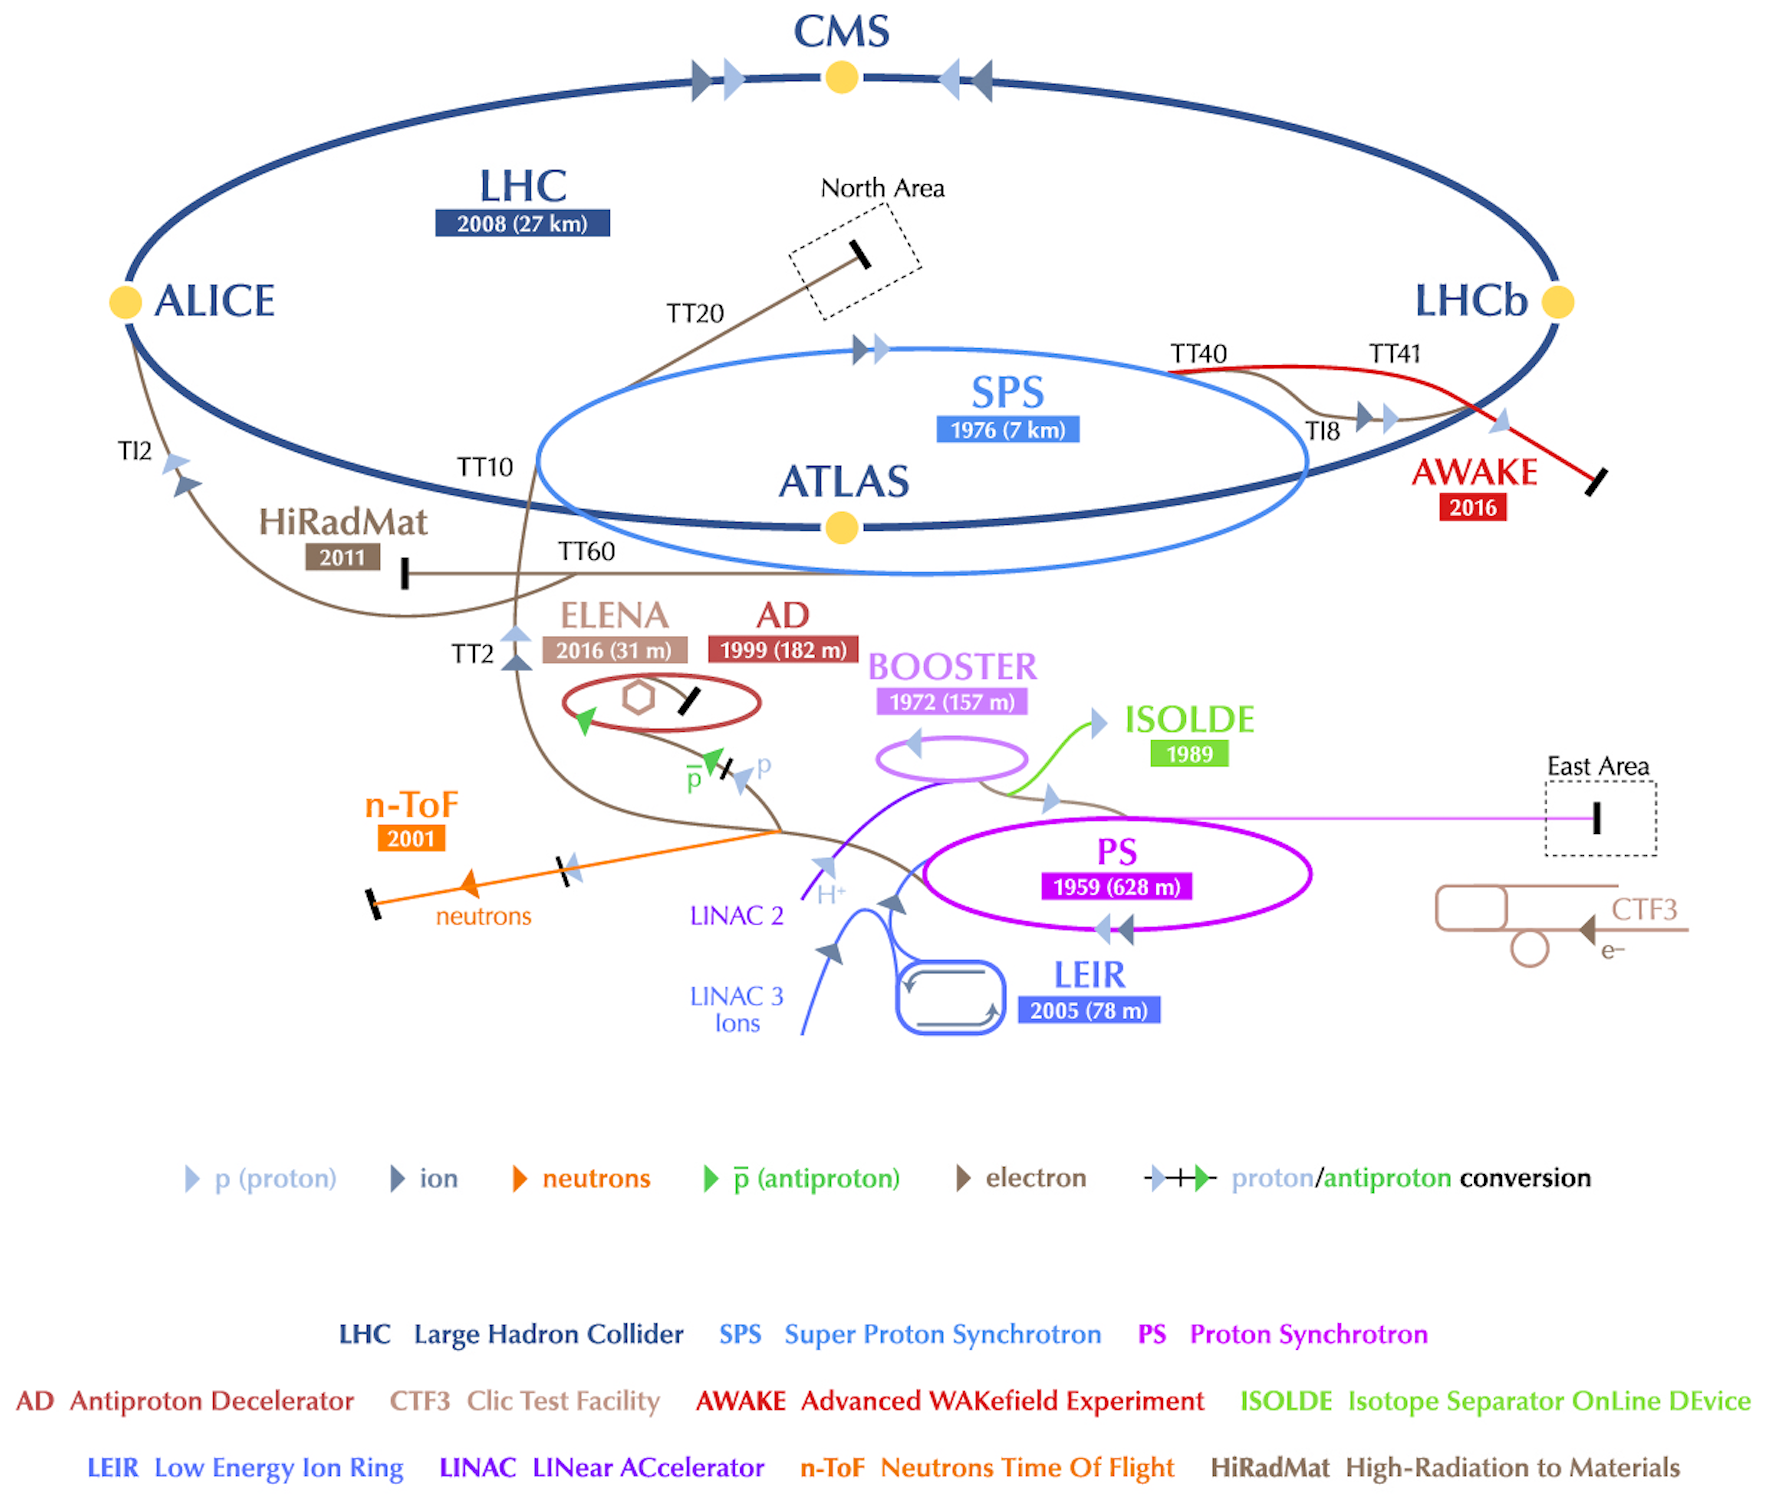
\includegraphics[width=0.9\columnwidth]{figures/detector/CERN_complex.png}
    \caption{The CERN accelerator complex, including the length and construction year for a number of accelerators, not all of which are used in $pp$ operations. During $pp$ operation, the proton acceleration chain is: LINAC 2 \to BOOSTER \to PS \to SPS \to LHC.  The figure is reproduced from Ref.~\cite{CERNcomplex}.}
    \label{fig:CERN_accerators}
\end{figure}

The LHC has been providing $pp$ collisions during two periods so far: Run~1 during 2011 and 2012, where the centre-of mass energies were $\sqrt{s}=7\tev$ and $8\tev$ respectively, and Run~2 from 2015 to 2018, where $\sqrt{s}=13\tev$. The instantaneous luminosity at the \lhcb collision point has been $4\times 10^{32} \cm^{-2} \,\mathrm s^{-1}$, and has allowed for the collection of a data set corresponding to an integrated luminosity of approximately 3\invfb during Run~1 and 6\invfb during Run~2. The full data set forms the basis of the thesis. This instantaneous luminosity is significantly lower than at other collision points, for example the peak instantaneous luminosity in the ATLAS detector was about $20\times 10^{33}\cm^{-2}\,\mathrm s^{-1}$ in 2018~\cite{ATLAS-CONF-2019-021},  50 times higher than in \lhcb. The lower luminosity is necessary to limit the number of $pp$ interactions per bunch crossing to an average of about 1.1--1.6 (depending on the data taking period), necessary for a vertex reconstruction with the required precision. The lower luminosity is achieved by colliding the proton beams with an off-set at the \lhcb collision point. This has the added benefit that the offset can be continuously adjusted during a fill of the LHC, and thus all data can be taken at the same instantaneous luminosity, allowing for simpler trigger configuration, and simpler subsequent analysis because the detector occupancy is constant. The lower luminosity, of course, comes with the downside that the collected data sample is smaller.

\begin{figure}[tb]
    \centering
    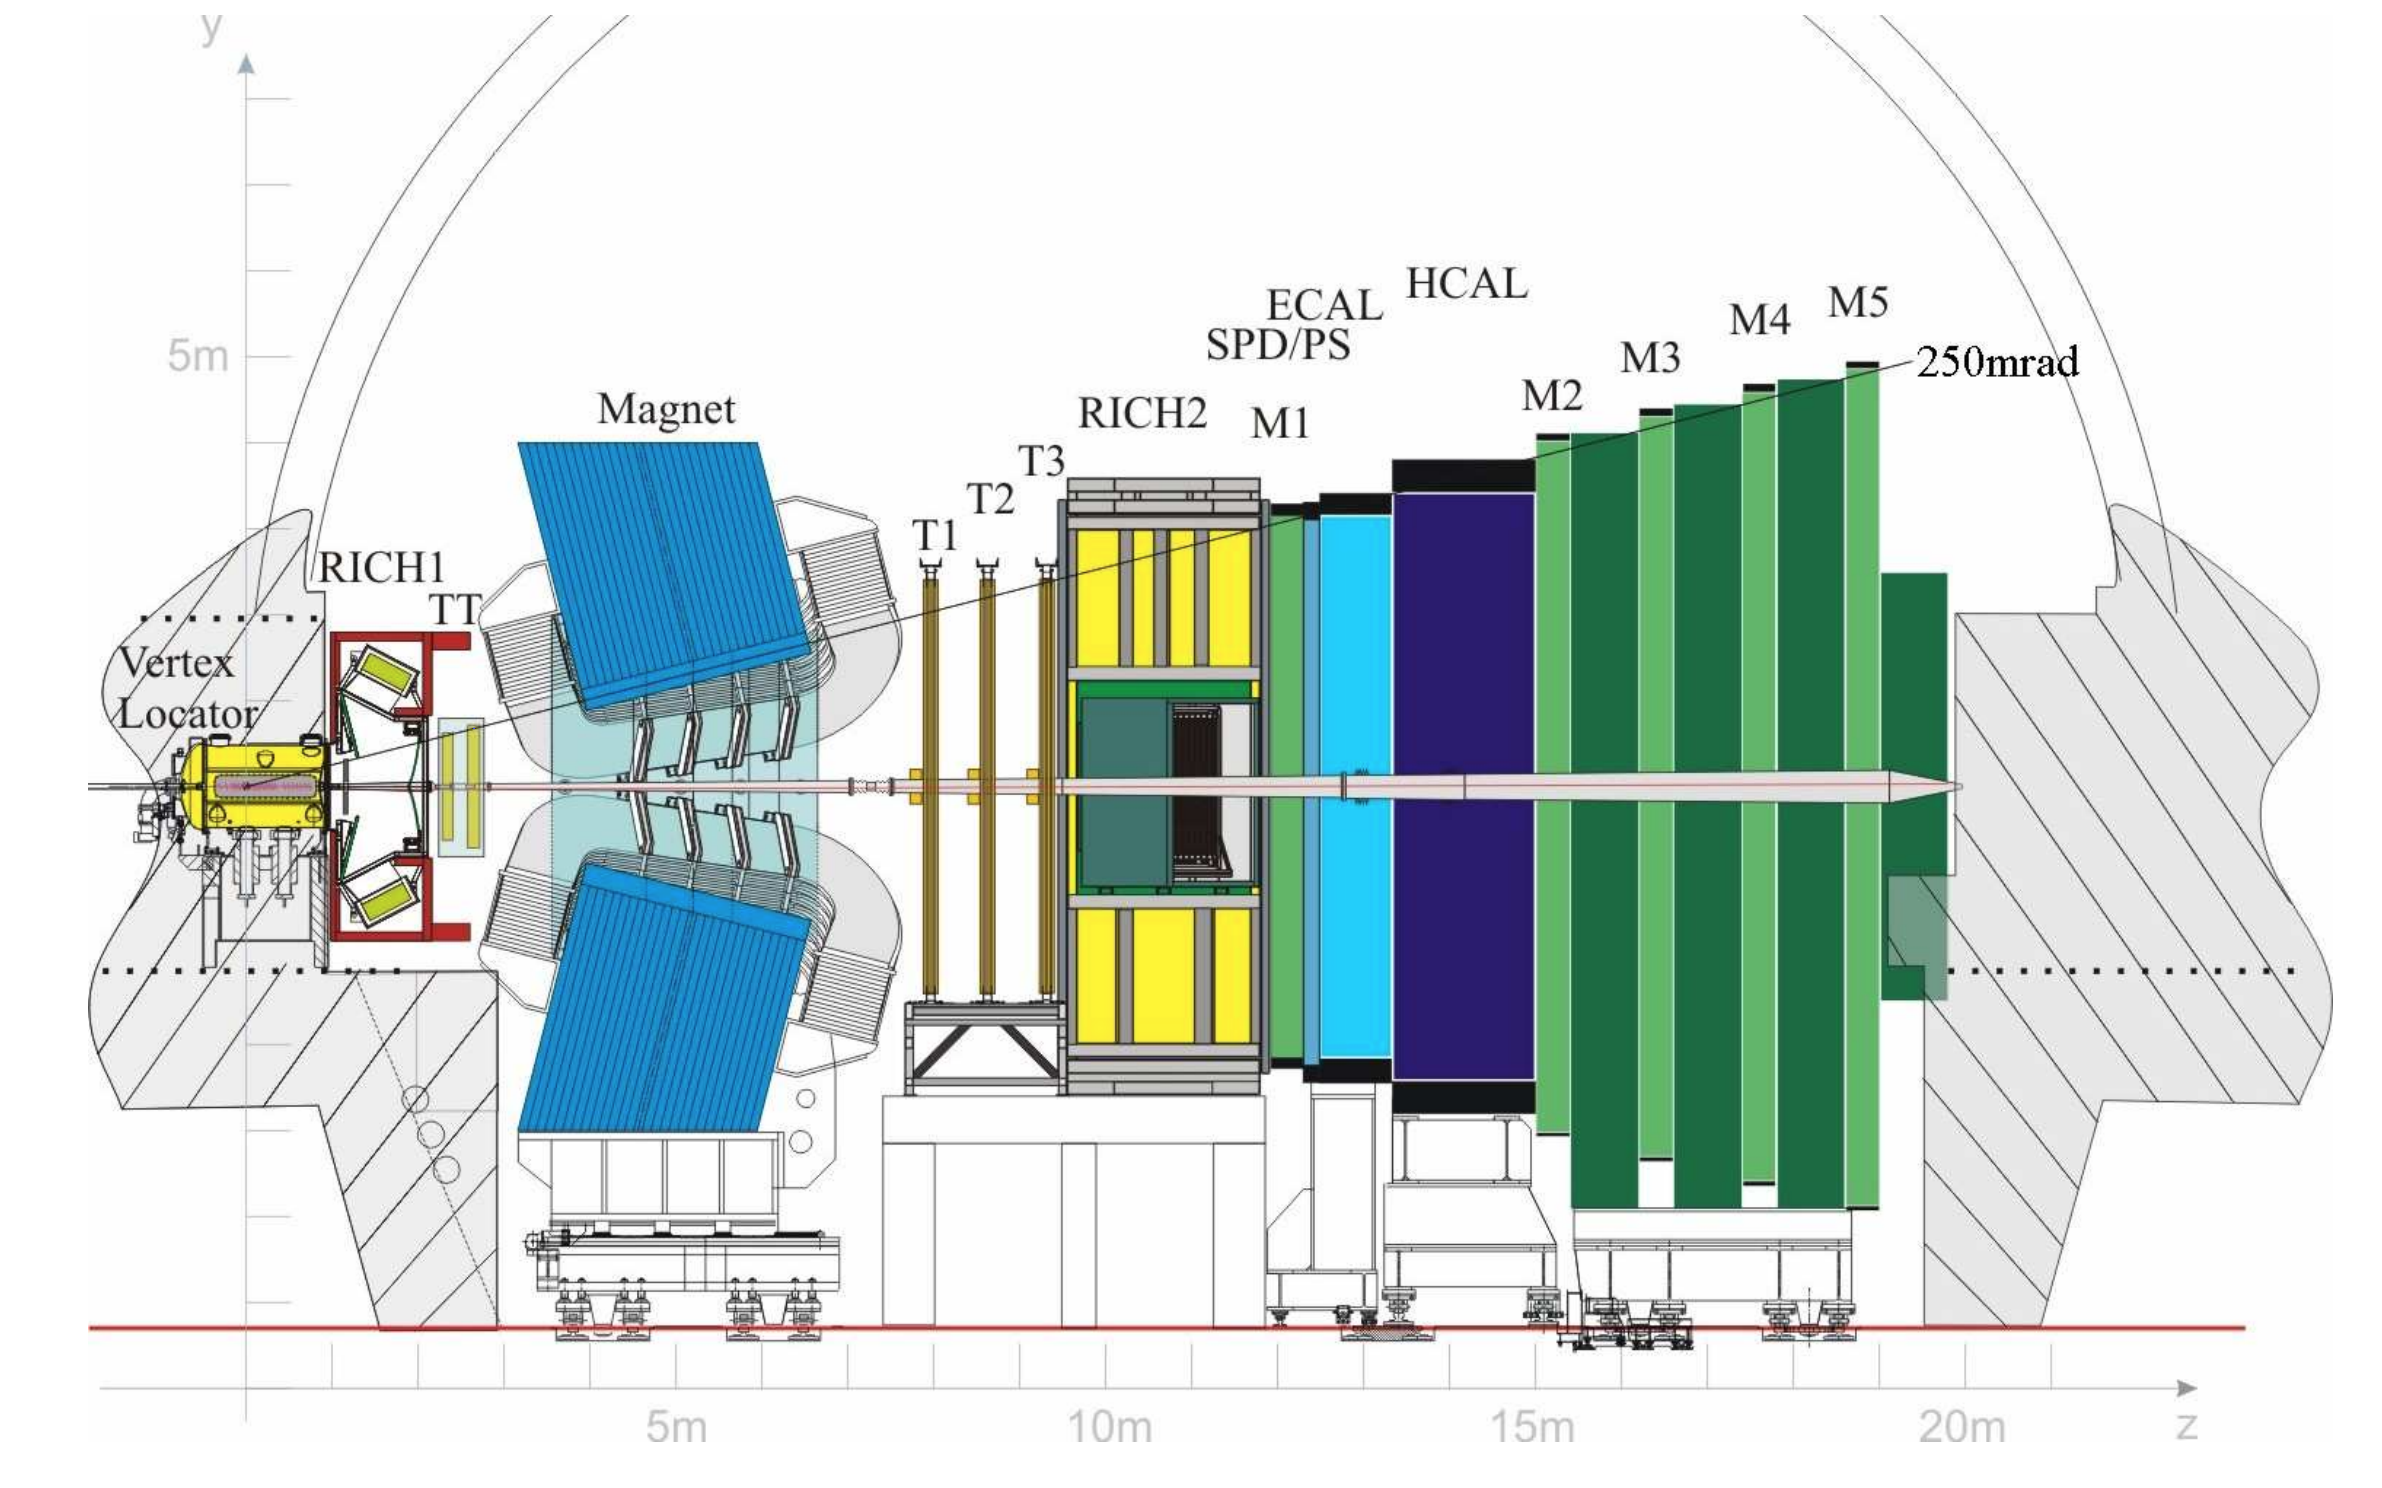
\includegraphics[width=\columnwidth]{figures/detector/LHCb_detector.png}
    \caption{Overview of the \lhcb detector reproduced from Ref.~\cite{LHCb-detector}. The individual subdetectors are described in detail in the text.}
    \label{fig:lhcb_detector}
\end{figure}



\section{The LHCb subdetectors} % (fold)
\label{sec:subdetectors}

\begin{figure}[tbp]
    \centering
    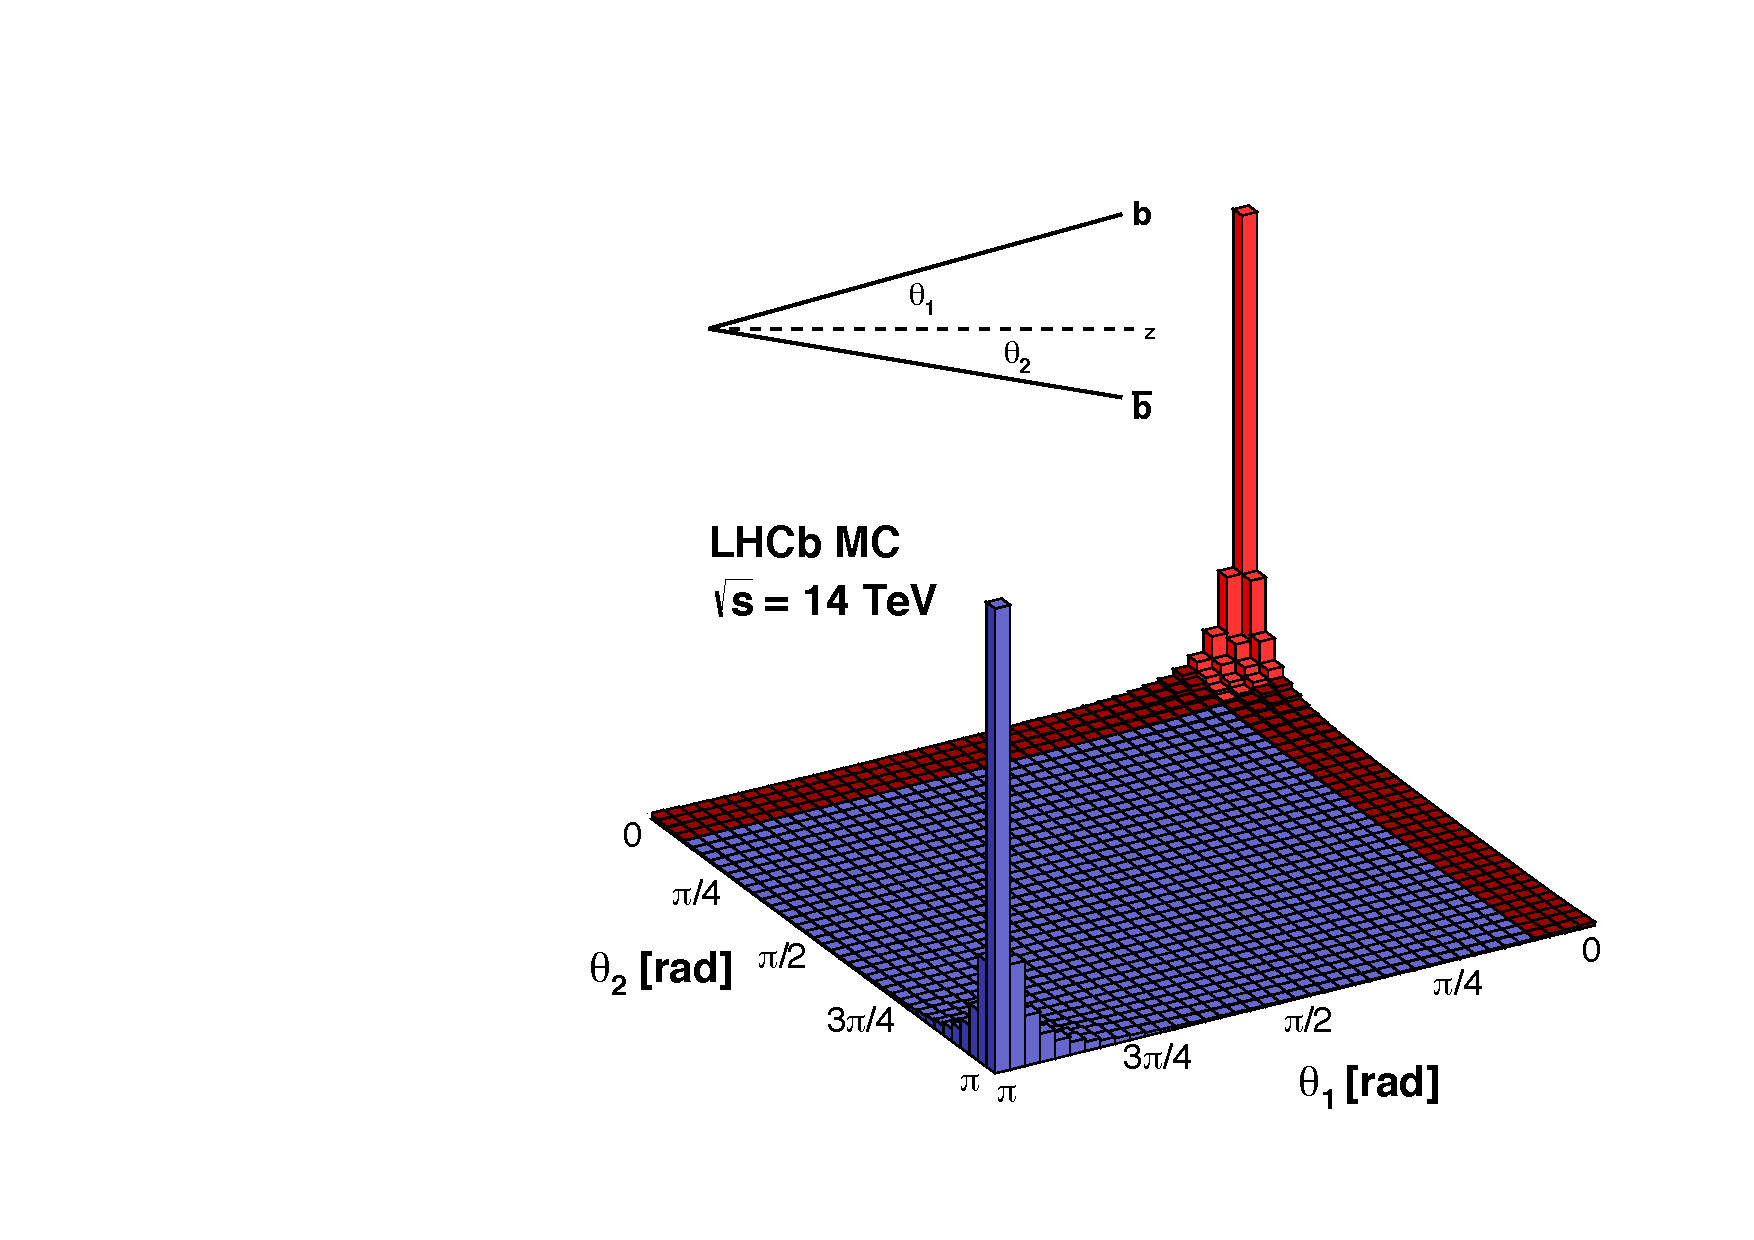
\includegraphics[width=0.8\columnwidth]{figures/detector/bbangles.pdf}
    \caption{Production cross section of $b\bar b$ pairs at a centre-of-mass energy of $\sqrt s = 14\tev$, as a function of $\theta_1$ and $\theta_2$, the angle of the $b$ and $\bar b$ quark, respectively, with respect to the beam axis $z$. The \lhcb acceptance is marked in red. The cross-section looks very similar for $\sqrt s = 7,\; 8,\; 13\tev$. The figure is taken from Ref.~\cite{bbangles}.}
    \label{fig:bb_angles}
\end{figure}

The \lhcb detector, shown in Fig.~\ref{fig:lhcb_detector},  is able to detect particles in the forward region $\eta\in[2, 5]$, corresponding to an angle $\theta$ with respect to the beam line between 15 and $300/250$\,mrad in the horizontal/vertical direction. As illustrated in Fig.~\ref{fig:bb_angles}, the $b\bar b$ production cross section is very large within the \lhcb acceptance: even though the acceptance covers less than 2\,\% of the solid angle,  24\,\% of all $b\bar b$ pairs created at $\sqrt{s}=14\tev$ are within the acceptance~\cite{bbangles} (for $\sqrt{s}=8\tev$ the number is 25\,\%). The detector is described with a coordinate system, where the $z$-axis is along the beam line and the $x$ $(y)$ axis is in the horizontal (vertical) directions normal to the beam line. The origin is at the collision point. The experiment consists of a number of sub detectors, located in the region from around the interaction point, and up to a distance of $z=20\,$m along the beam line (in the following, the direction from the interaction point towards the sub detectors is denoted \emph{downstream}, and the opposite direction \emph{upstream}). This section describes each of them in detail.
 
\subsection{The VELO} % (fold)
\label{sub:the_velo}
The VErtex LOcator (VELO)~\cite{VELO-TDR} is a silicon detector located immediately around the collision point, used to provide precise measurements of the particle track coordinates in the interaction region. These are used to reconstruct the production and decay vertices of beauty and charm hadrons with a very high accuracy,  and play an important role in the full track reconstruction. The ability to distinguish tracks originating in secondary vertices also plays a crucial role in efficient triggering, as described further below.

The detector consists of 21 VELO stations positioned along the beam line as illustrated in Fig.~\ref{fig:VELO_stations}. Each station consists of two \emph{modules}, mounted on each side of the beam line; each module, in turn, consists of two silicon strip detectors,  where the strips are oriented to provide a measurement of $r$, the radial distance from the beam line, and  $\phi$, the azimuthal angle, respectively. This is illustrated in Fig.~\ref{fig:VELO_sensors}. The strip pitch varies between 40 and $100\,\mu$m depending on the distance from the beam line.  The stations are positioned such that all tracks that are within the acceptance region of the downstream detectors and originate at the interaction point are guaranteed to intersect 3 detector stations. During operation, the segments are located only 8\mm from the beam; this is achieved by mounting them on a moving frame that can be retracted during beam commissioning to avoid radiation damage. The detectors are kept in a vacuum, shielded from the beam vacuum by a $0.3\mm$ thick \emph{RF foil} made of aluminium that also serves to screen the detector from electric fields induced by the proton beam. The silicon sensors were kept at an operating temperature of about -7\,C$^\circ$, achieved with a liquid-CO$_2$ cooling system.

\begin{figure}[tbp]
    \centering
    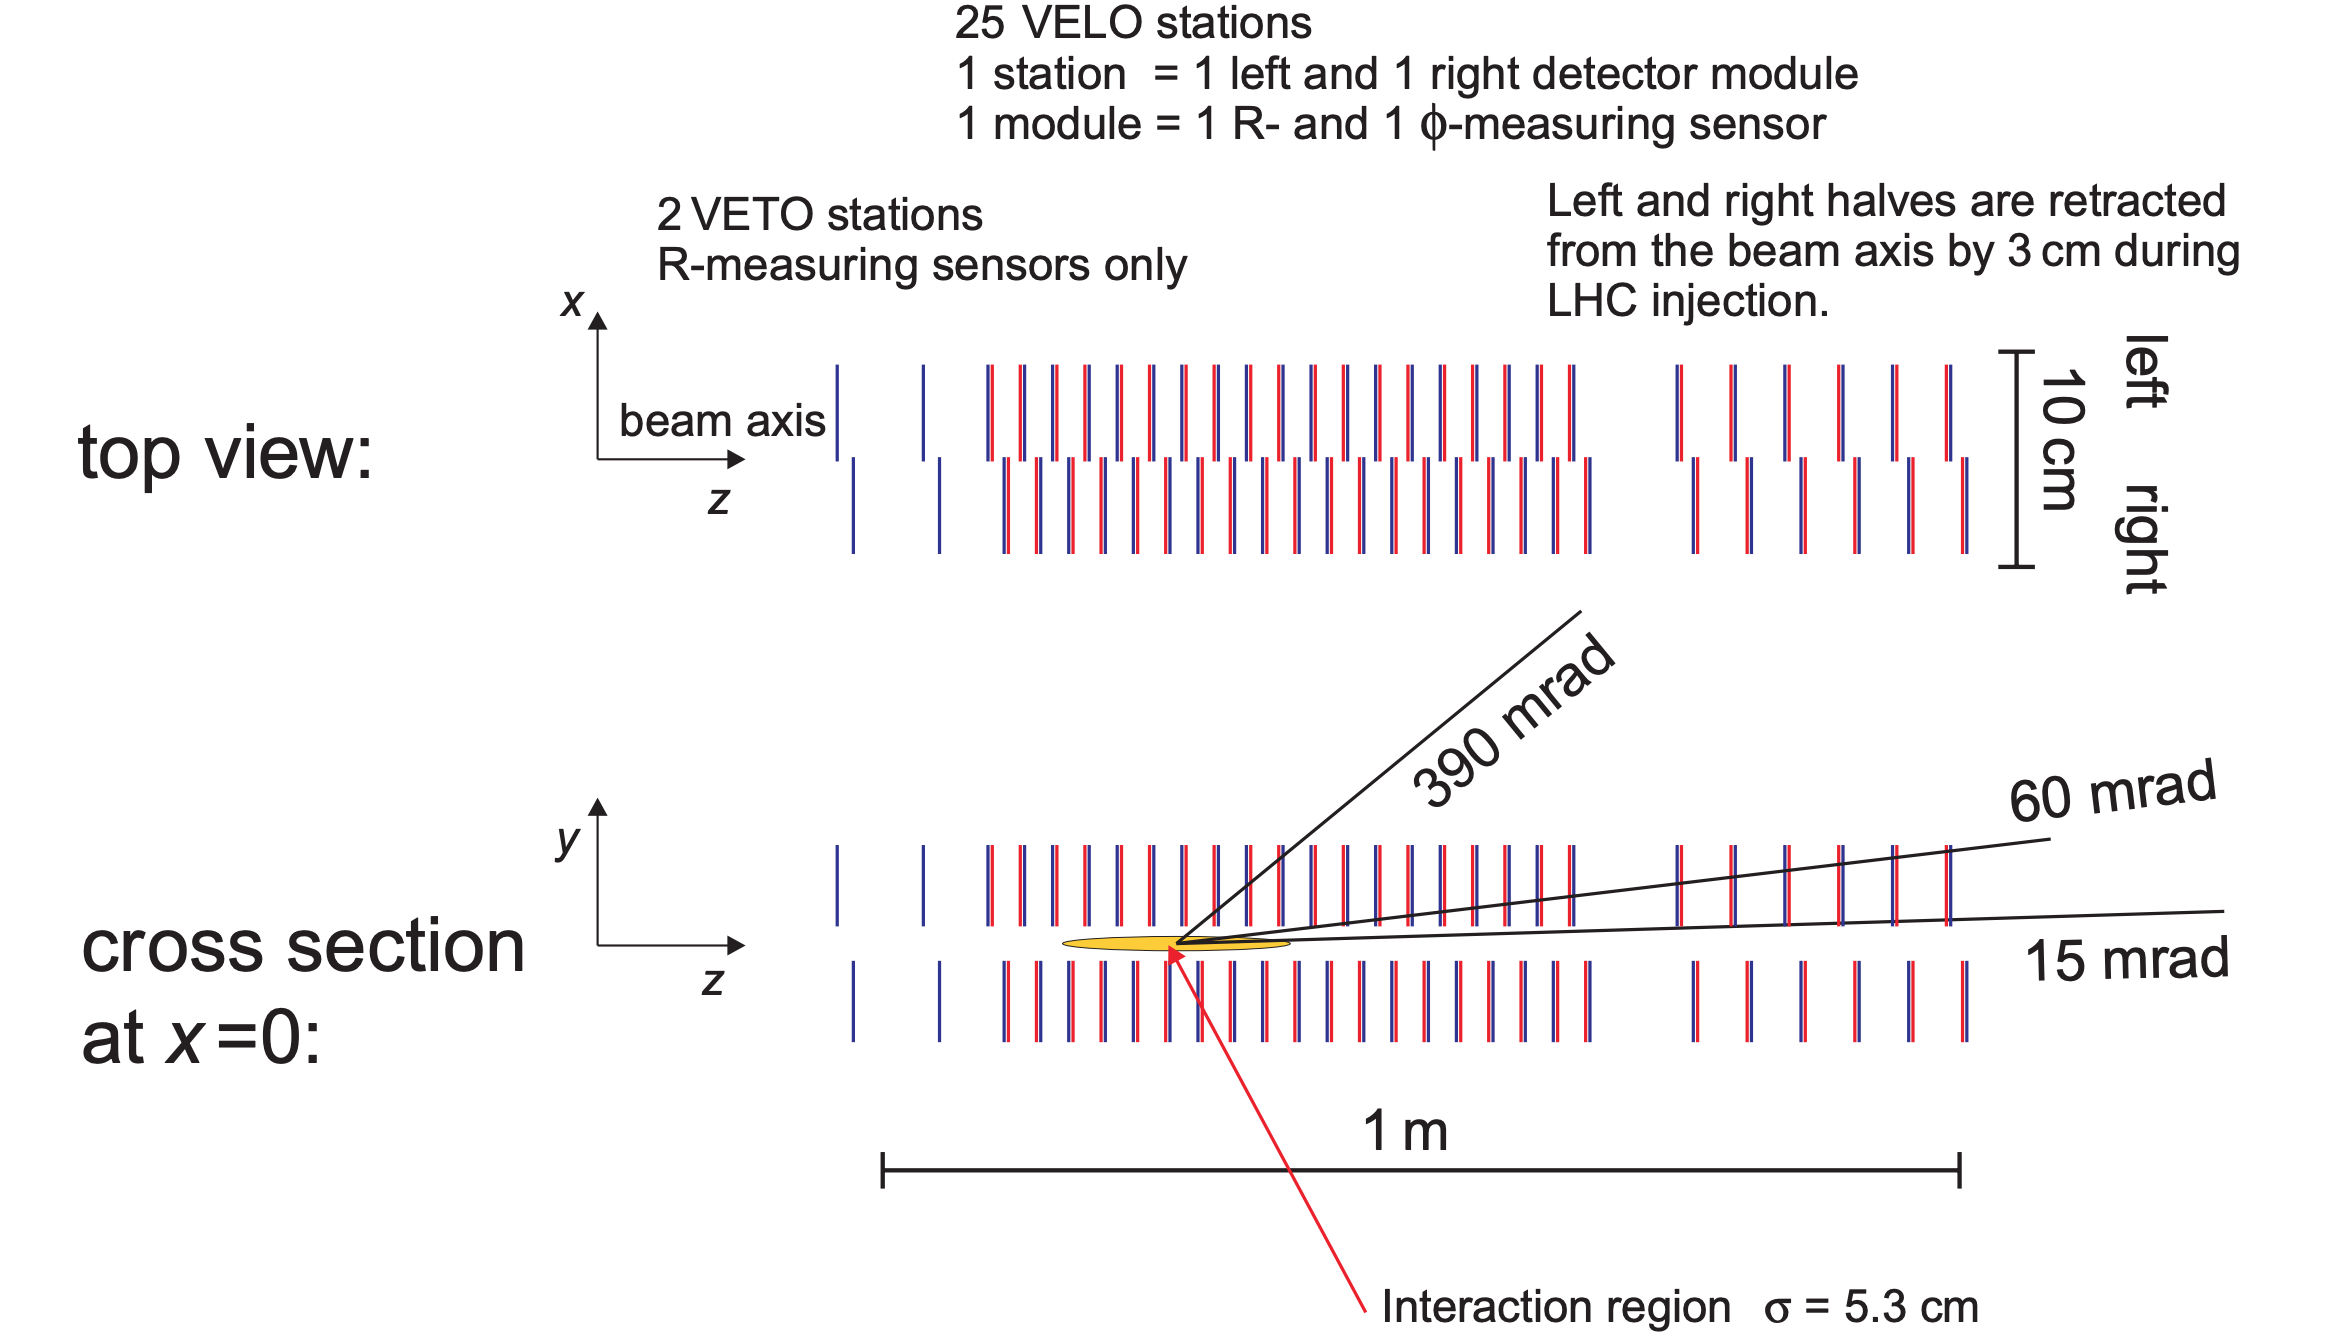
\includegraphics[width=0.95\columnwidth]{figures/detector/VELO_stations.png}
    \caption{Overview of the arrangement of VELO stations from the VELO Technical Design Report (TDR)~\cite{VELO-TDR}. The actual detector includes 21 stations instead of 25, but the overall design is identical~\cite{VELO-Performance}.}
    \label{fig:VELO_stations}
\end{figure}

\begin{figure}[tb]
    \centering
    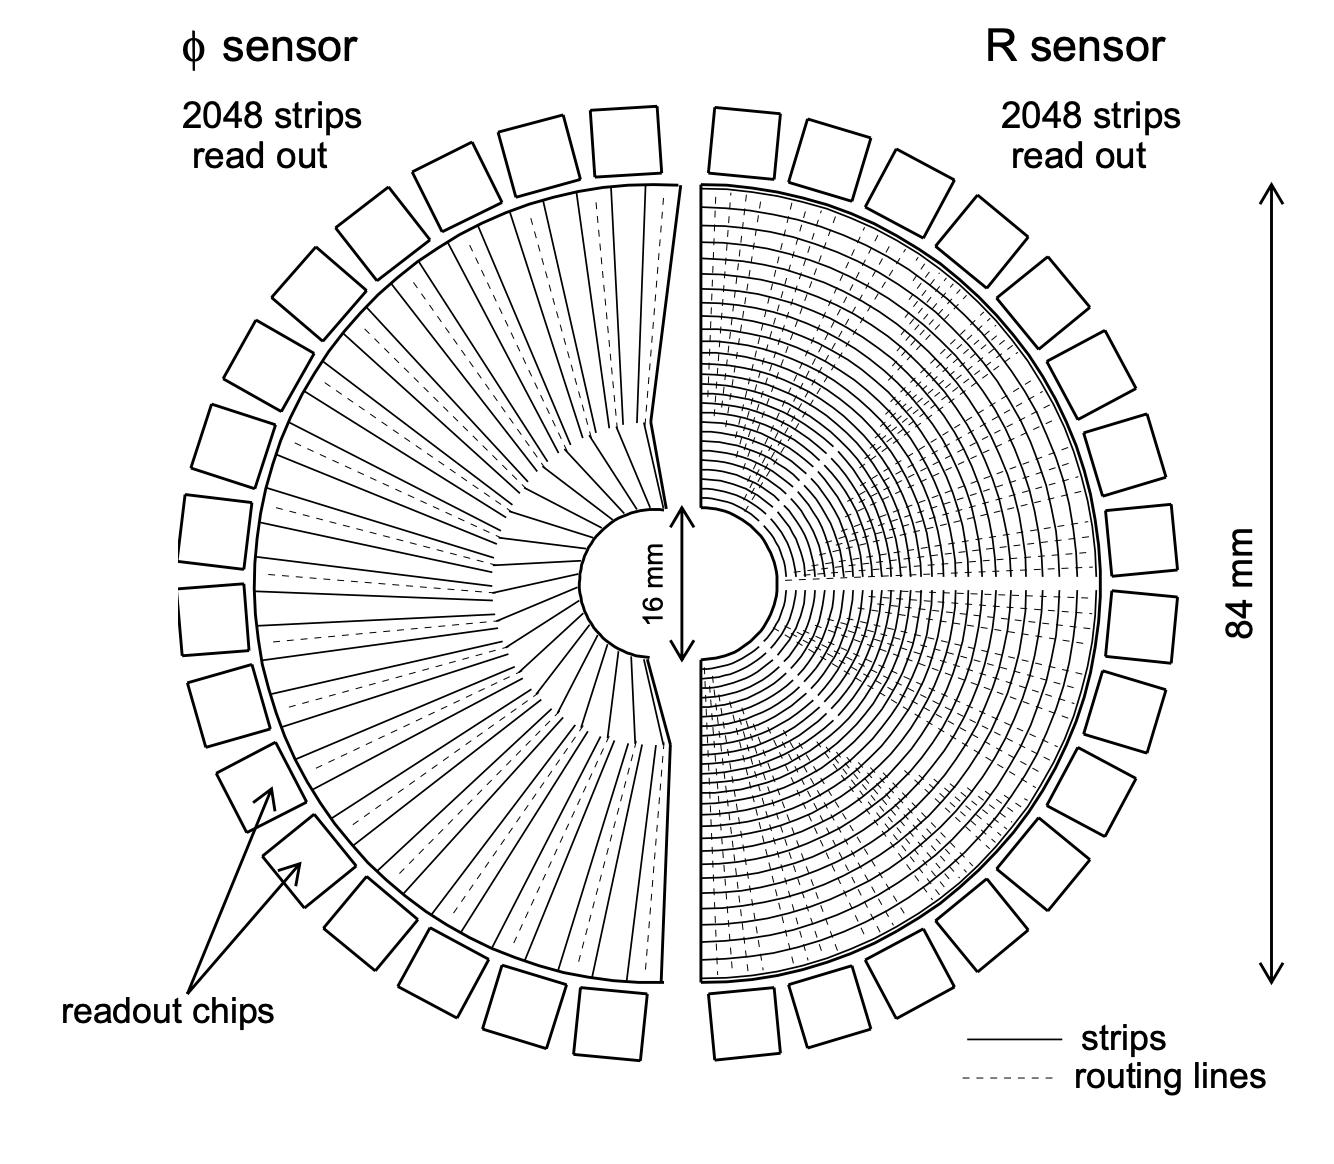
\includegraphics[width=0.55\columnwidth]{figures/detector/VELO_sensors.png}
    \caption{Illustration of the silicon strip layout in the VELO modules designed to measure (left) the azimuthal angle, $\phi$, of a track, and (right) the radial distance from the beam, $r$. Reproduced from Ref.~\cite{VELO-TDR}.}
    \label{fig:VELO_sensors}
\end{figure}

The primary vertex (PV) resolution of the VELO is typically $\sim $10\mum in the $x$ and $y$ directions and $\sim$50\mum in the $z$ direction, improving with the number of tracks originating at the PV, and deteriorating with the overall number of PVs~\cite{VELO-Performance}. The typical uncertainty on the decay length of a \B meson is about $230\mum$, compared to a typical decay length of $\mathcal O(10)\mm$. The resolution of the \emph{impact parameter}, IP, of a track is well-described by the formula $\sigma_\mathrm{IP}=(15+29/[p_T/(\gev/c)])\mum$. This parameter excellently distinguishes particles produced in secondary decays, from those produced in the primary interaction (for which the IP would be zero, were it not for the experimental resolution).
% subsection the_velo (end)

\subsection{Magnet and tracking stations} % (fold)
\label{sub:magnet_and_tracking_stations}

The \lhcb experiment uses a warm (non-superconducting) dipole magnet to measure the momentum of charged particles, by providing a maximum magnetic field strength of approximate $1\T$ and a total bending power of about $4\,$T\,m over the region where $z\in[2.5, 8]\m$. The magnetic field has been measured to a relative precision of about $4\times 10^{-4}$ and is uniform in the $x$ and $y$ planes to within a percent within the tracking volume~\cite{LHCb-detector}. The profile of the magnetic field along the $z$-axis is shown in Fig.~\ref{fig:track_types} on page~\pageref{fig:track_types}, where the track types within \lhcb are defined. The magnet can provide a magnetic field in either vertical direction; over the span of a year of running the experiment approximately equal amounts of data are collected with the magnet in the "Up" and "Down" configurations; this leads to the cancellation of a number of charge-asymmetry effects, significantly reducing potential systematic uncertainties. 

The tracking system consists of the VELO, and four other tracking stations: the Tracker Turicencis (TT) upstream of the magnet, and the tracking stations 1--3 (T1, T2, T3) downstream of the magnet. The downstream tracking stations each consist of an Inner Tracker (IT) based on silicon strips, and an Outer Tracker (OT) that employs drift tubes. 

\begin{figure}[tb]
    \centering
    \begin{subfigure}{0.55\columnwidth}
        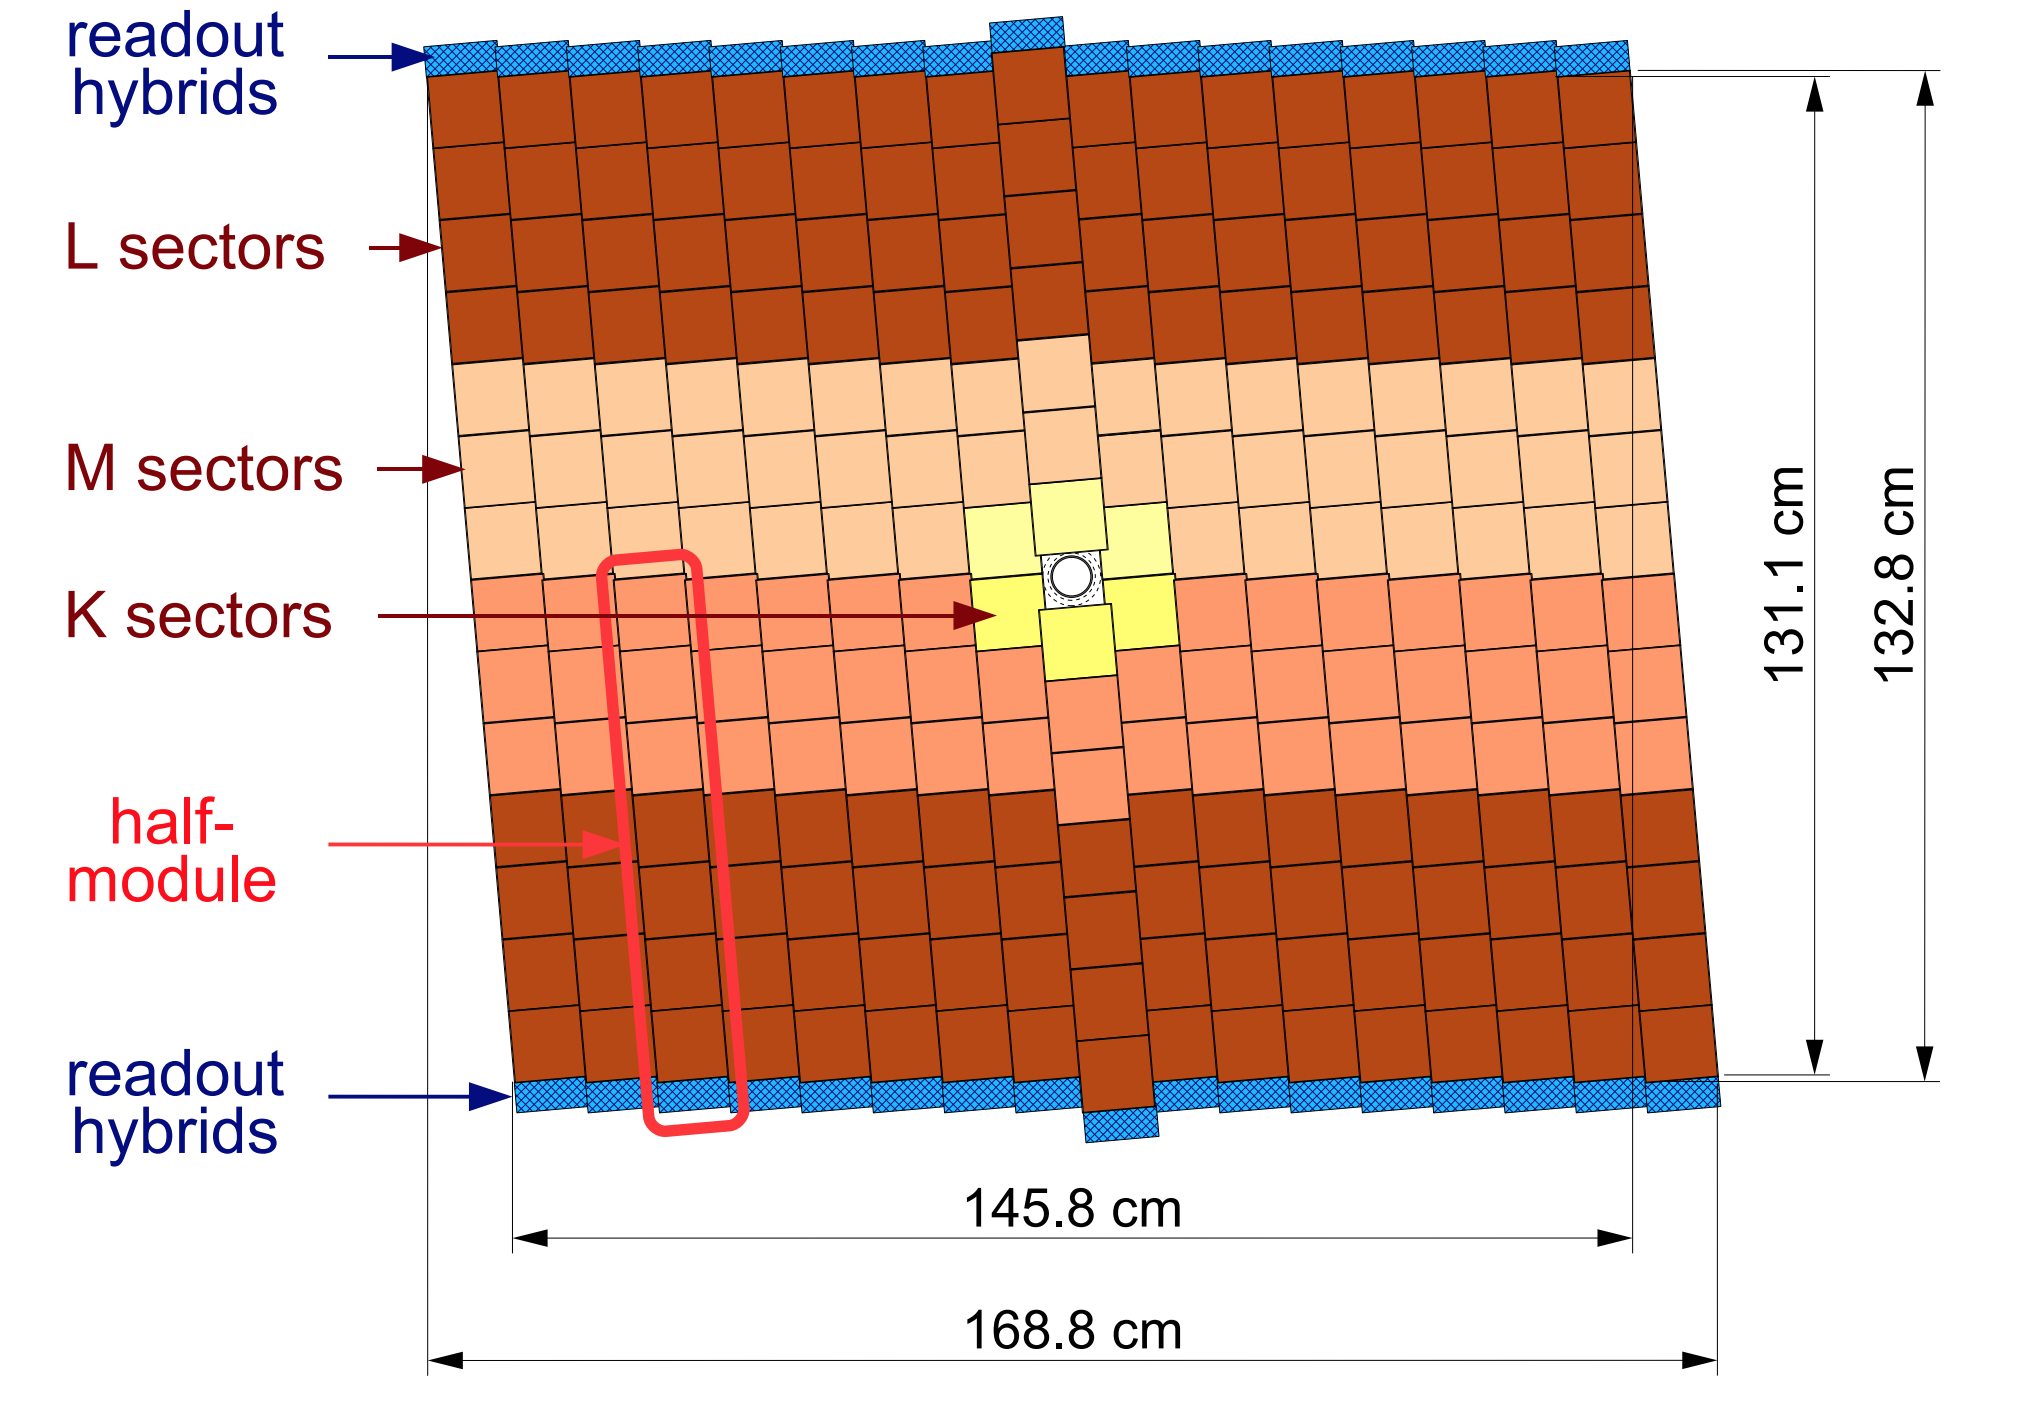
\includegraphics[width=\columnwidth]{figures/detector/TT_station.png}
        \caption{\label{fig:TT_station}}
    \end{subfigure}
    \begin{subfigure}{0.42\columnwidth}
        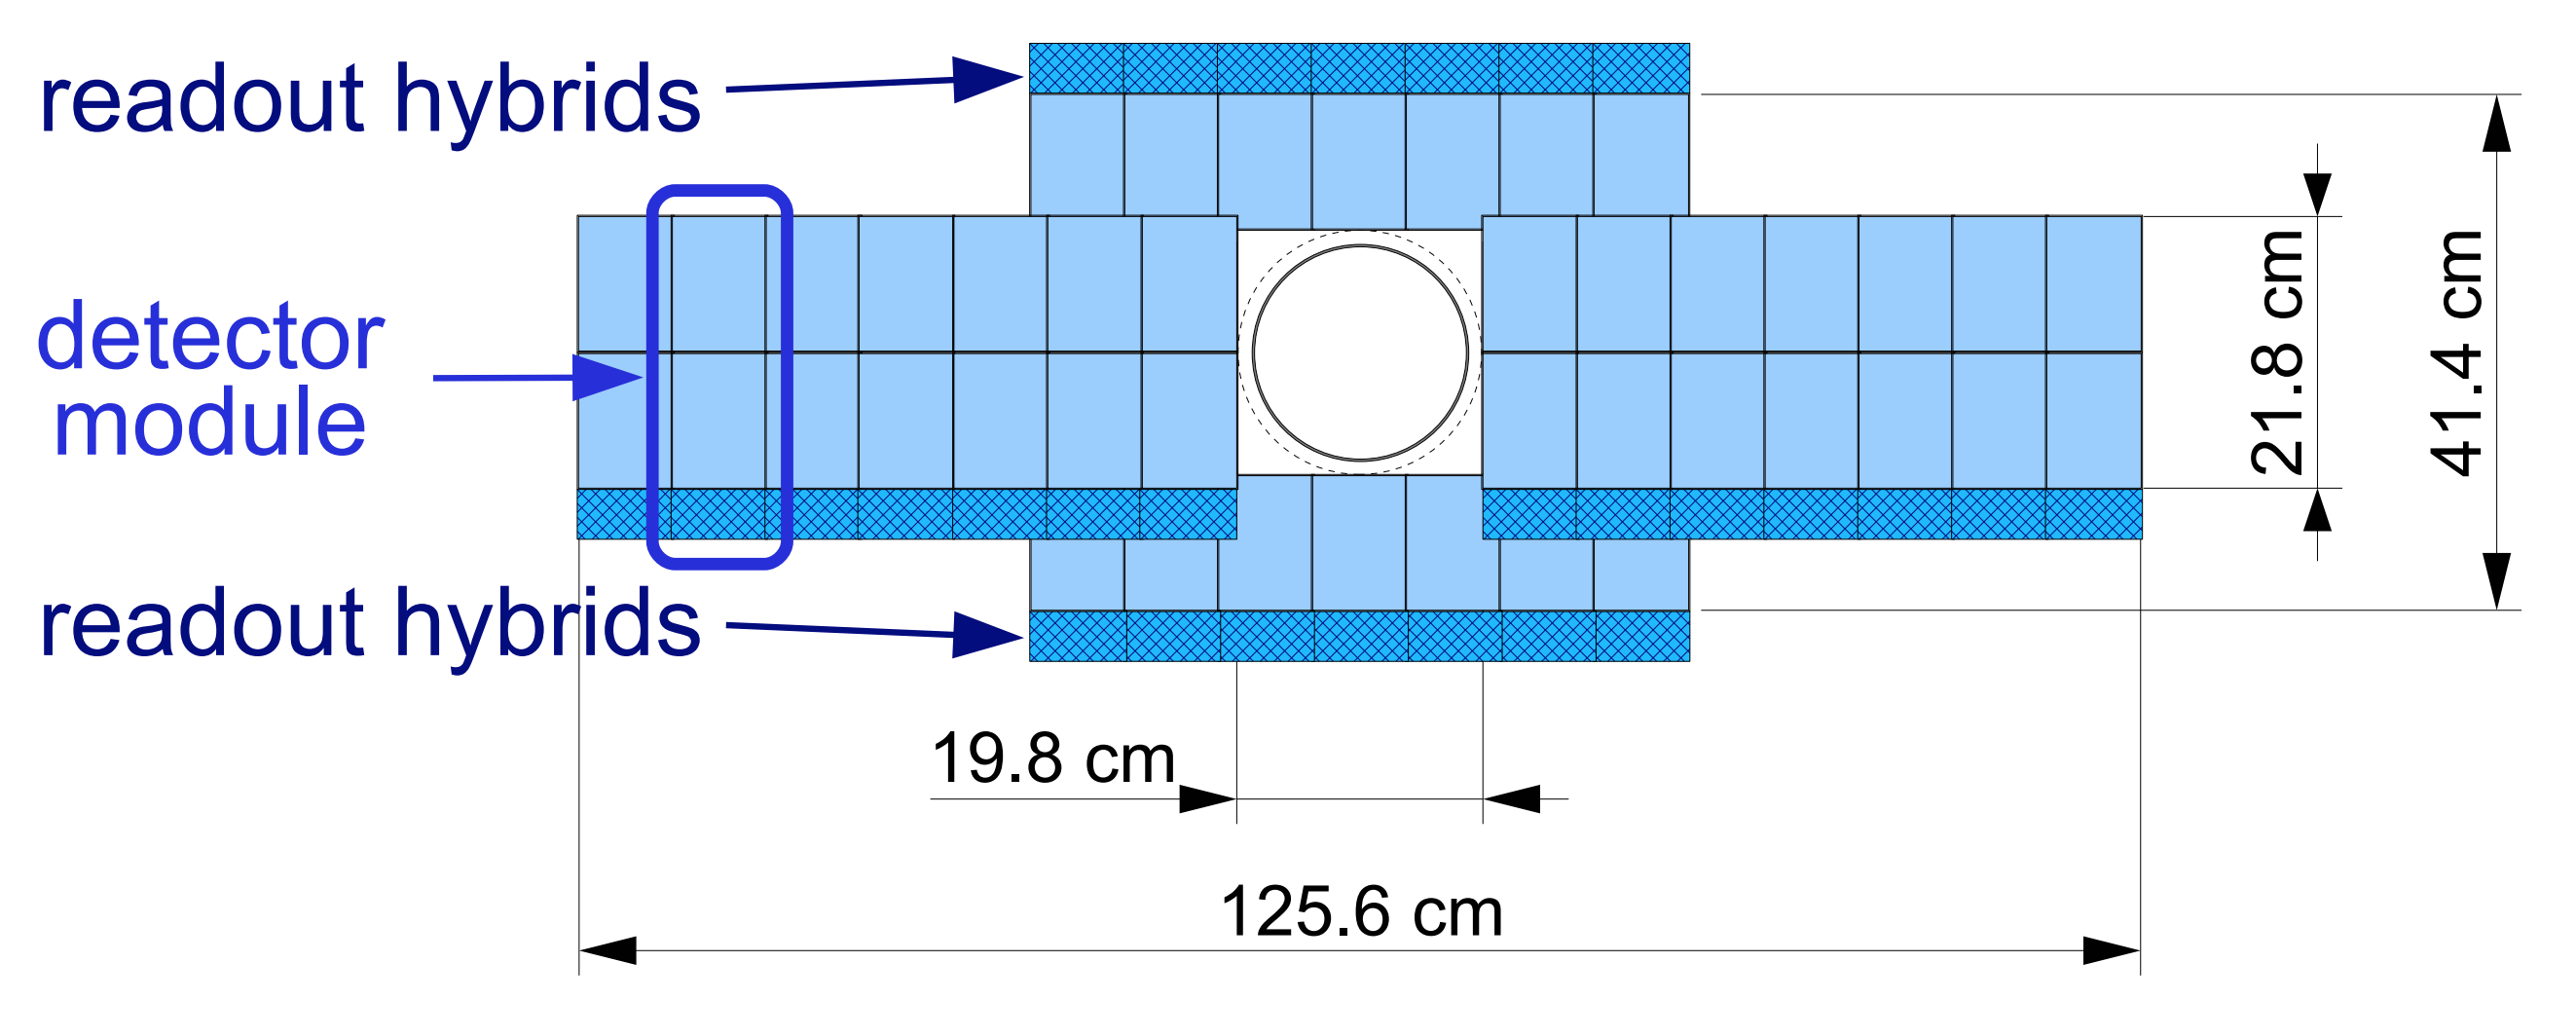
\includegraphics[width=\columnwidth]{figures/detector/IT_station.png}
        \caption{\label{fig:IT_station}}
    \end{subfigure}
    \caption{Overview of (a) a $v$-layer module of the TT and (b) and $x$-layer module of the IT. Reproduced from Ref.~\cite{LHCb-detector}}
    \label{fig:TT_IT_stations}
\end{figure}

Both the TT and IT are based on silicon strip detectors with a pitch of about $200\mum$; they were developed as a single project and are collectively known as the Silicon Tracker (ST). The TT  is a 140\cm wide and 130\cm tall planar tracking station, covering the whole \lhcb acceptance. It is shown in Fig.~\ref{fig:TT_station}. At each of the T1--T3 stations,  the IT consist of four modules, arranged around the beam pipe as illustrated in Fig.~\ref{fig:IT_station}. They do not cover the full \lhcb acceptance, only the very-forward region where the number of tracks is largest. Each TT or IT module comprises of four layers of silicon strips, where the central two layers are rotated $\pm5^\circ$ with respect to the first and last layer (an $x$-$u$-$v$-$x$ geometry). The ST has a spatial resolution for a given track of approximately 50\mum, chosen because the overall momentum resolution is then dominated by multiple-scattering effects for almost all reconstructed tracks.

\begin{figure}[tb]
    \centering
    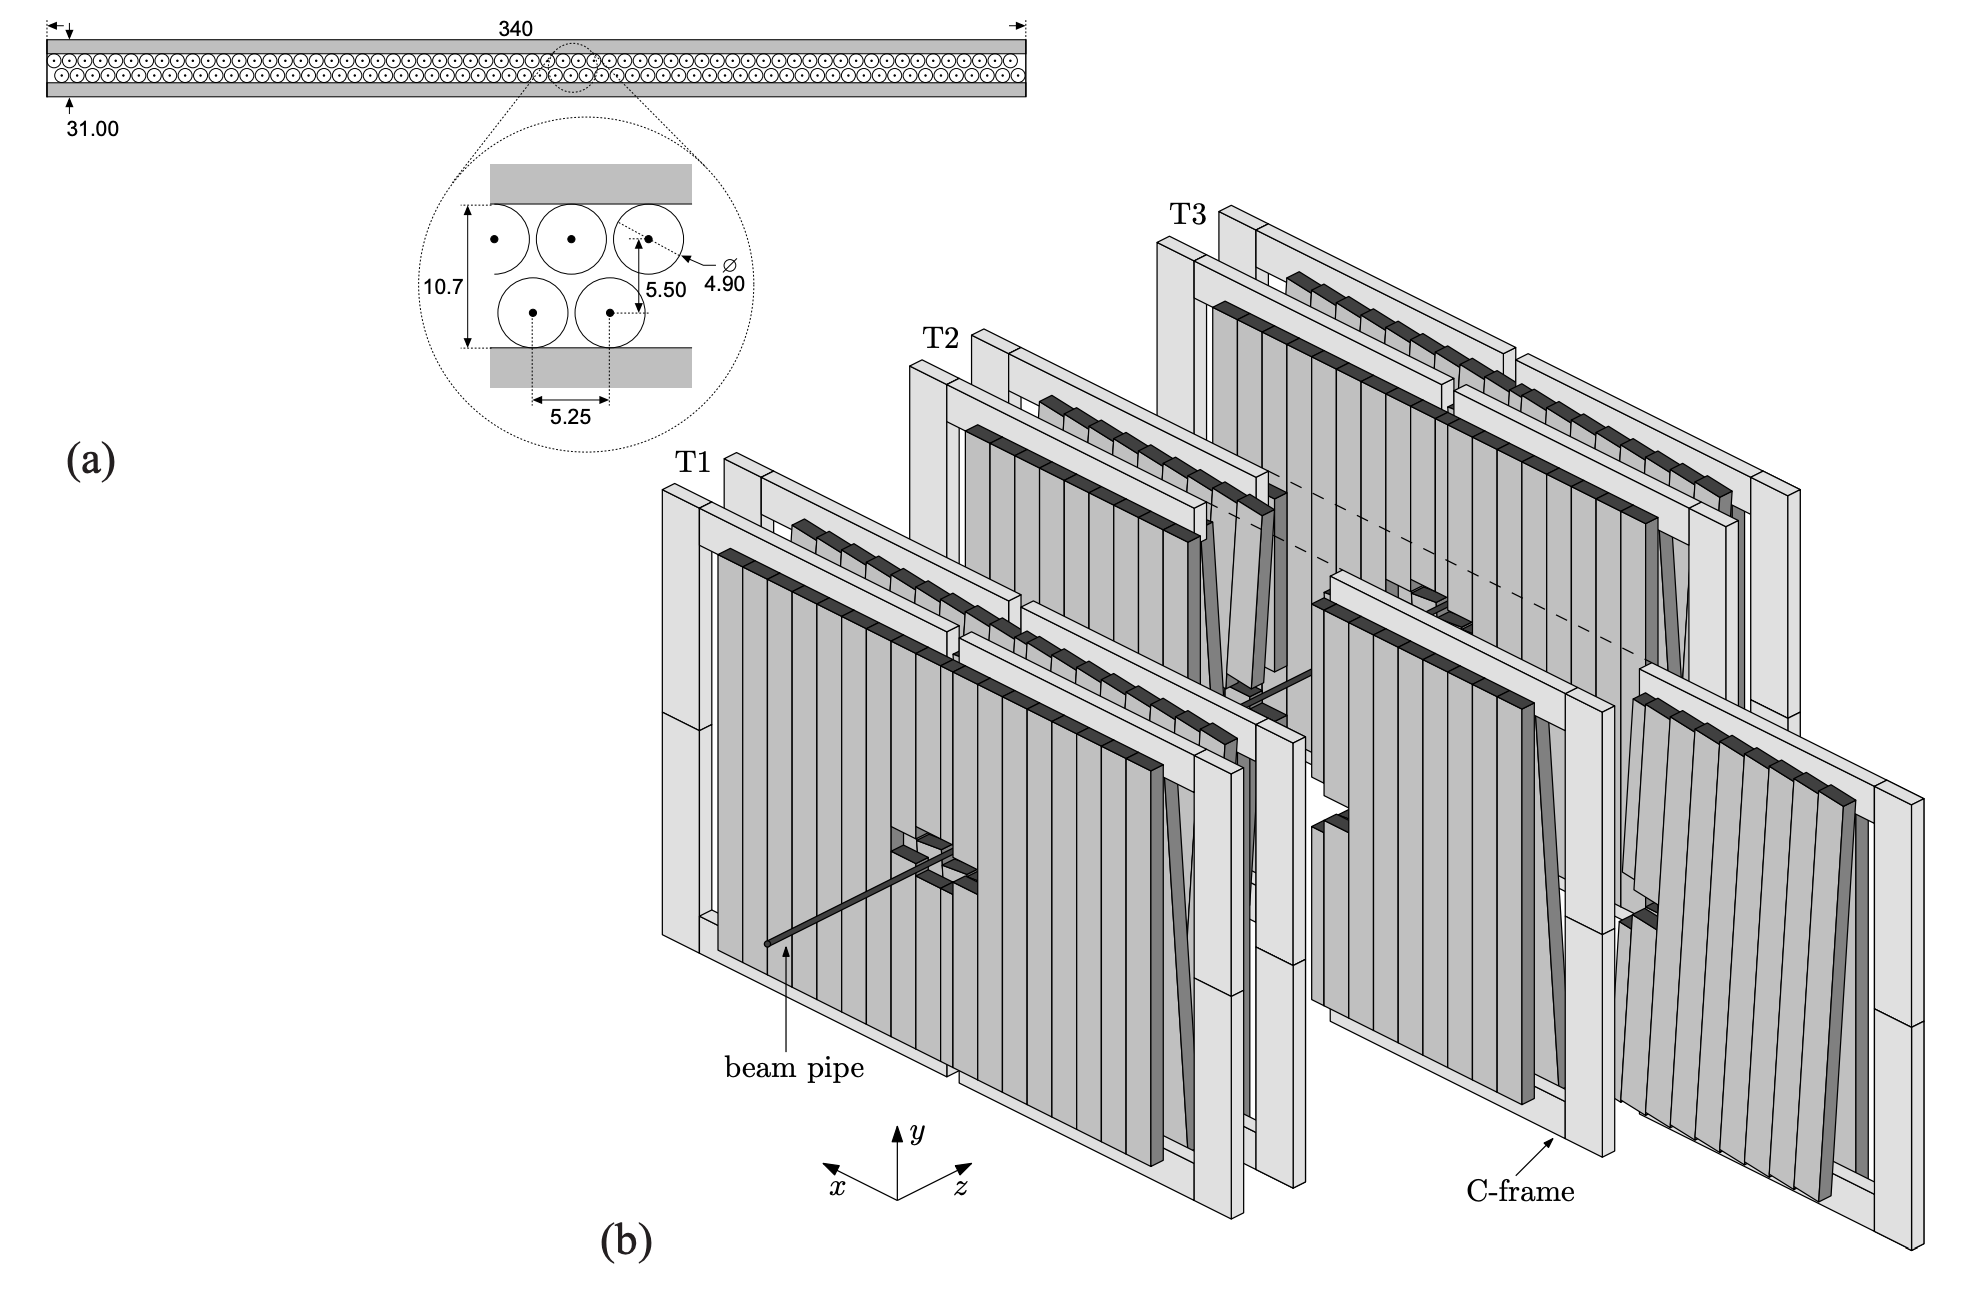
\includegraphics[width=\columnwidth]{figures/detector/OT_stations.png}
    \caption{(a) Cross section of an OT module. (b) Arrangement of the OT modules in tracking stations. Reproduced from Ref.~\cite{OT-Performance}.}
    \label{fig:OT_station}
\end{figure}

At the T1--T3 stations, the OT covers the part of the overall acceptance of 300 (250)\,mrad in the horizontal (vertical) plane that is not covered by the IT. The OT consists of arrays of gas-tight drift tubes with inner diameters of 4.9\mm. The OT is shown illustrated in Fig.~\ref{fig:OT_station}. An Ar/CO$_2$/O$_2$ (70/28.5/1.5) gas mixture is used to fill the tubes that ensures a drift time below 50\ns and a drift coordinate resolution of 200\mum. The use of a drift-chamber detector is necessary, because it was not economically feasible to instrument the whole \lhcb acceptance with silicon strip detectors in T1--T3. The condition that the OT occupancy should not be above 10\,\% in the planned run conditions determined the boundary between the IT and the OT (in practice, the \lhcb has been running at twice the original design luminosity so the actual occupancy has been higher). 

\begin{figure}[tb]
    \centering
    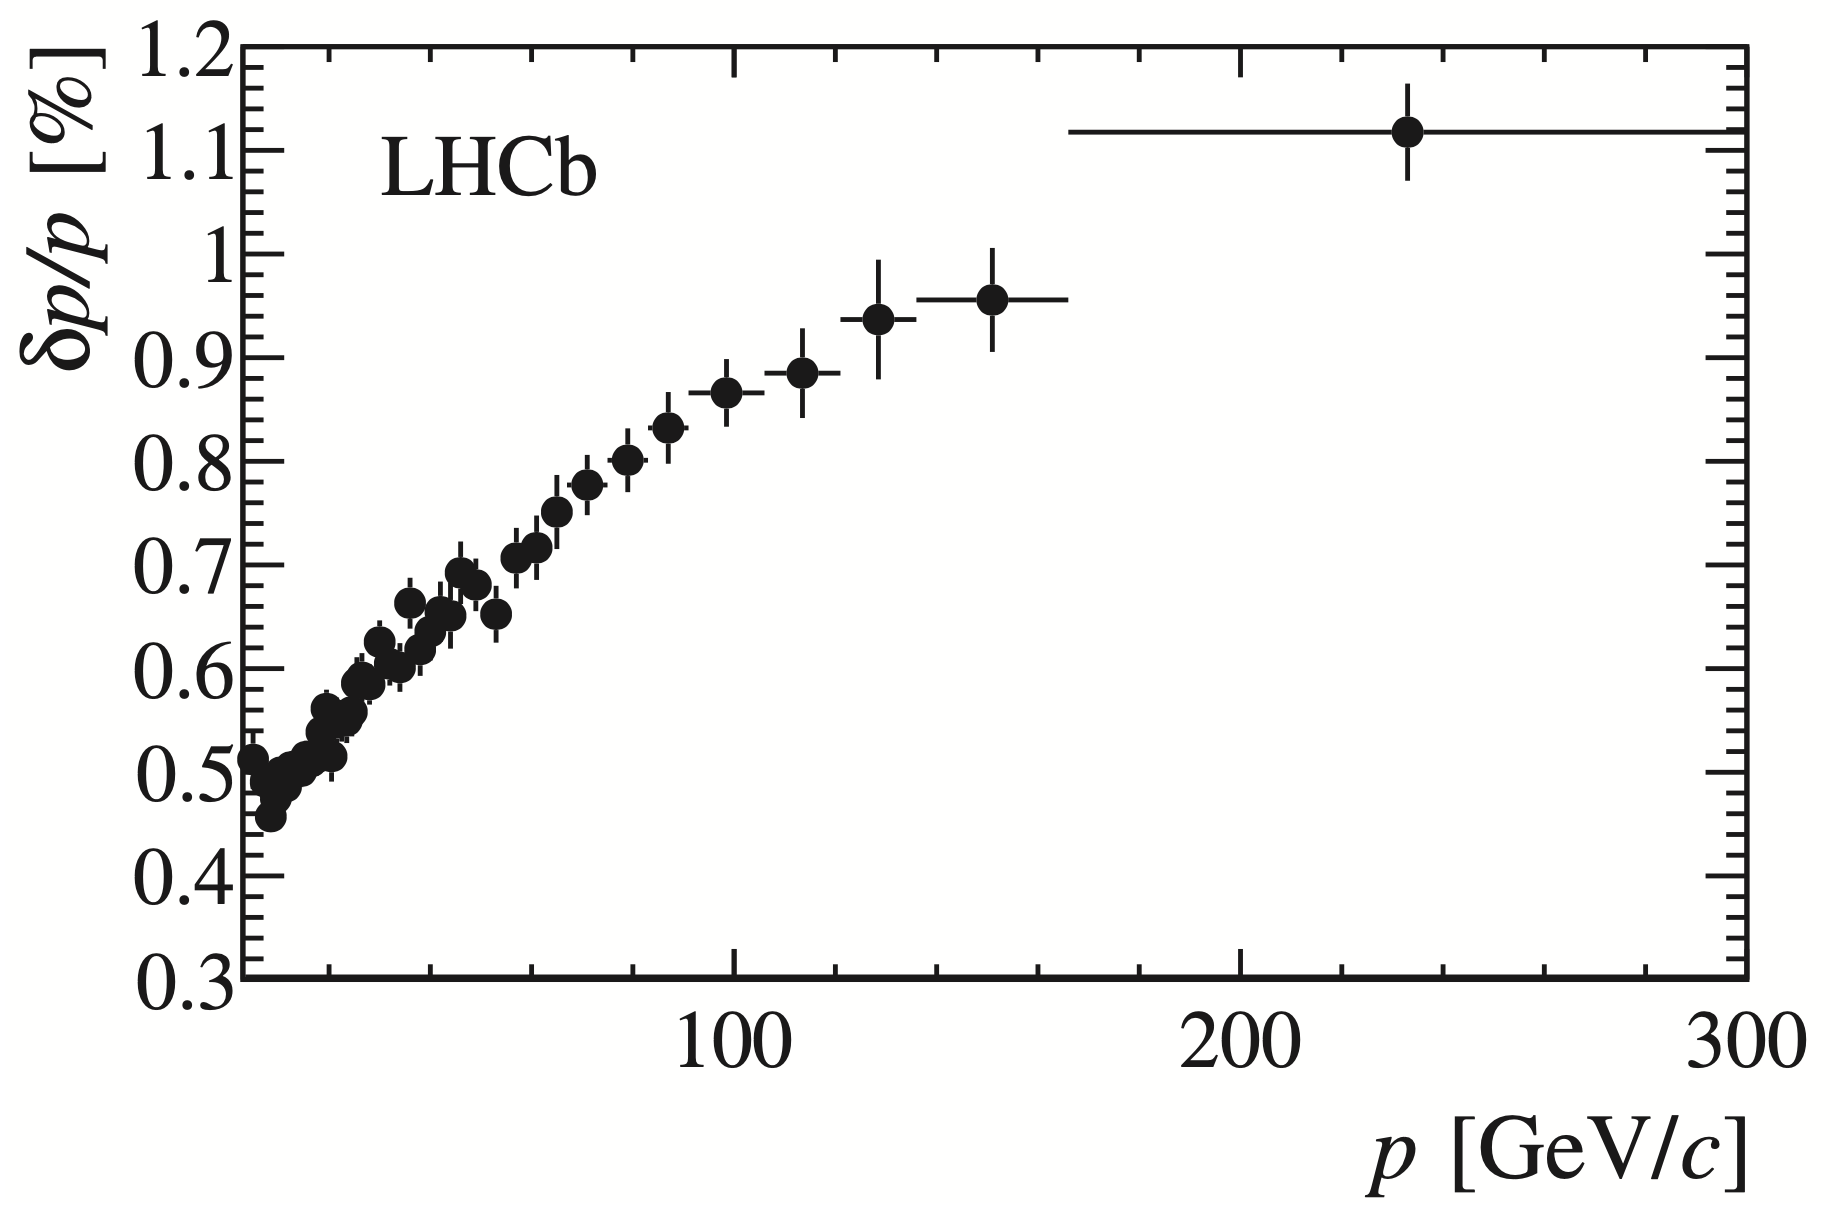
\includegraphics[width=0.55\columnwidth]{figures/detector/momentum_resolution.png}
    \caption{Relative uncertainty on the momentum of charged tracks (specifically long tracks, cf. the definitions in Section~\ref{sec:reconstruction}) in the \lhcb detector, determined via the mass resolution obtained in $J/\psi\to\mup\mu^-$ decays in Run~1 data. Reproduced from Ref.~\cite{LHCb-Performance}}
    \label{fig:momentum_resolution}
\end{figure}

The overall relative momentum resolution achieved for most charged tracks in \lhcb is less than a percent, as illustrated in Fig.~\ref{fig:momentum_resolution}, where it has been determined from a fit to the mass peak in $J/\psi\to\mup\mu^-$ decays in Run~1 data. 

% subsection magnet_and_tracking_stations (end) 

\subsection{The RICH detectors} % (fold)
\label{sub:the_rich}

\begin{figure}[tb]
    \centering
    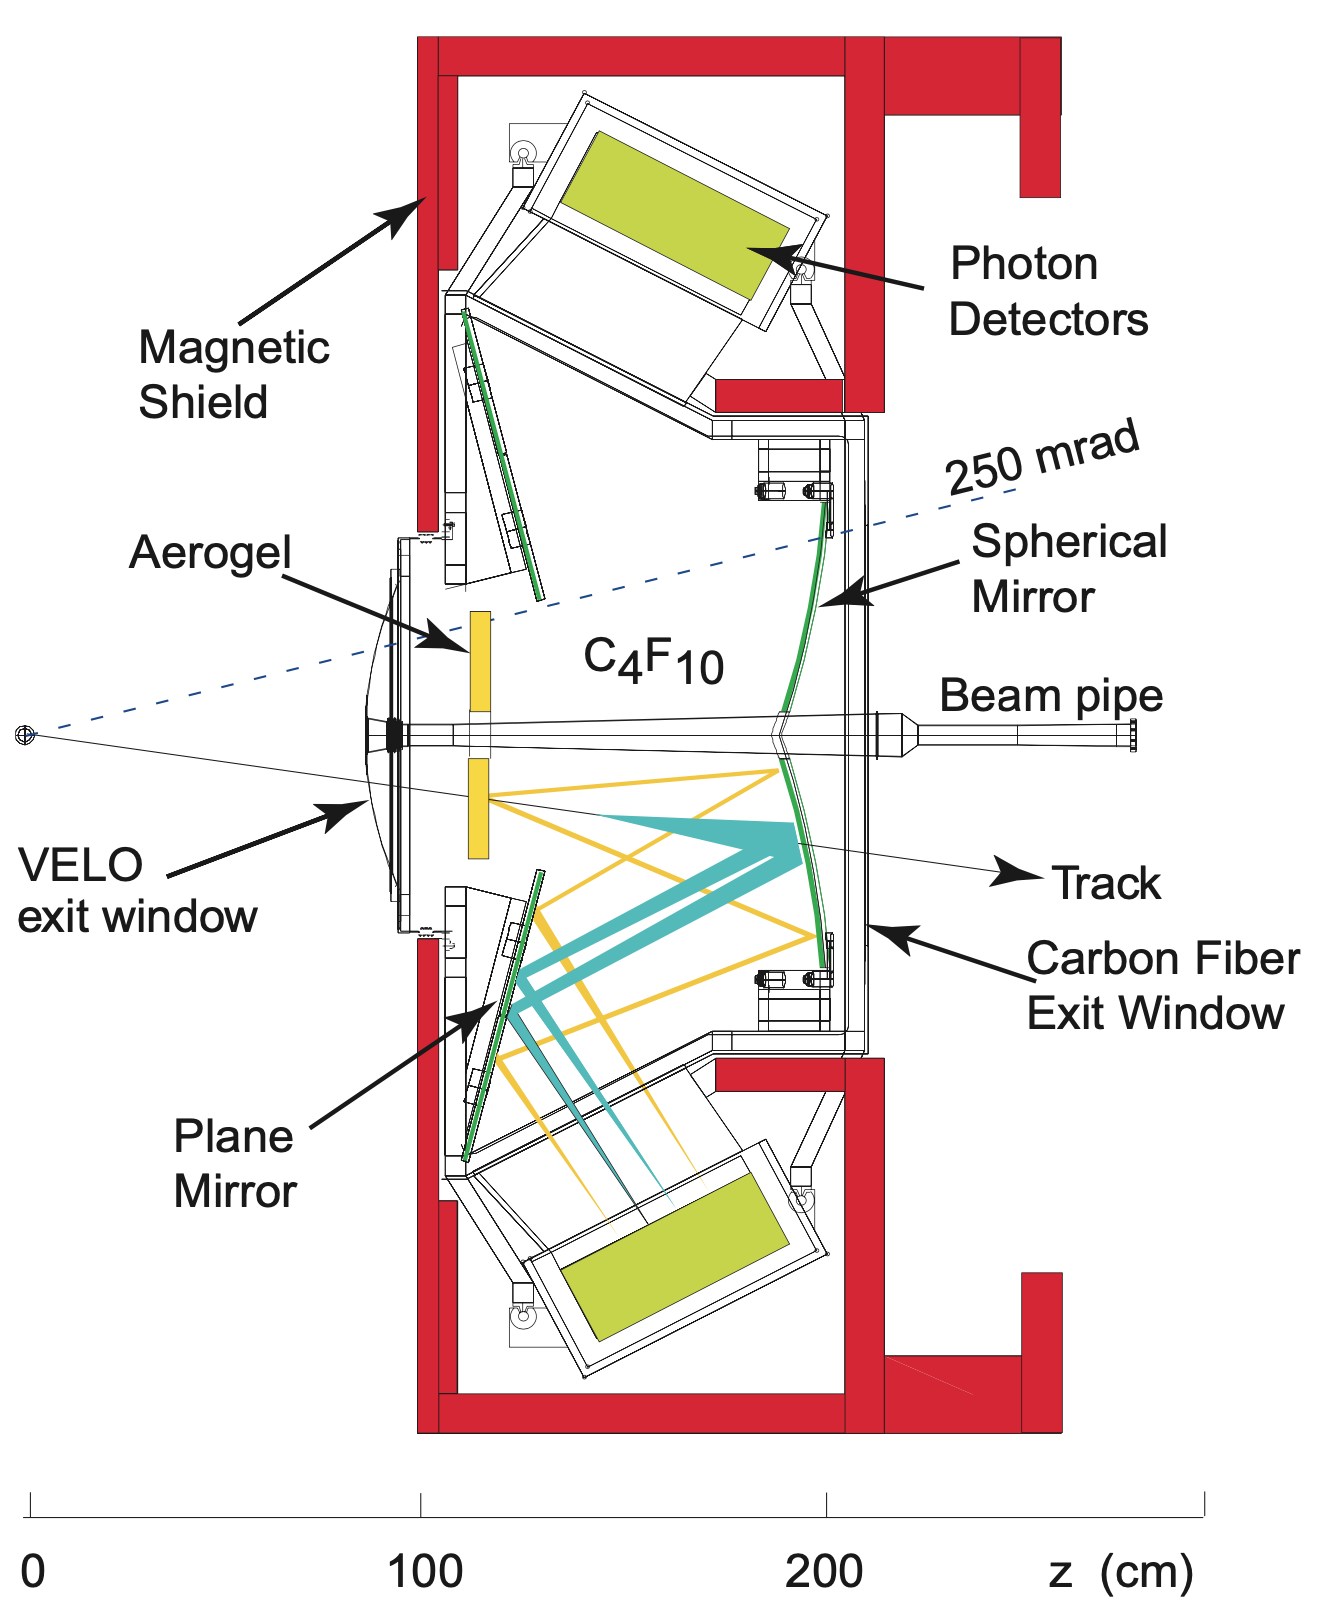
\includegraphics[width=0.45\columnwidth]{figures/detector/RICH1.png}
    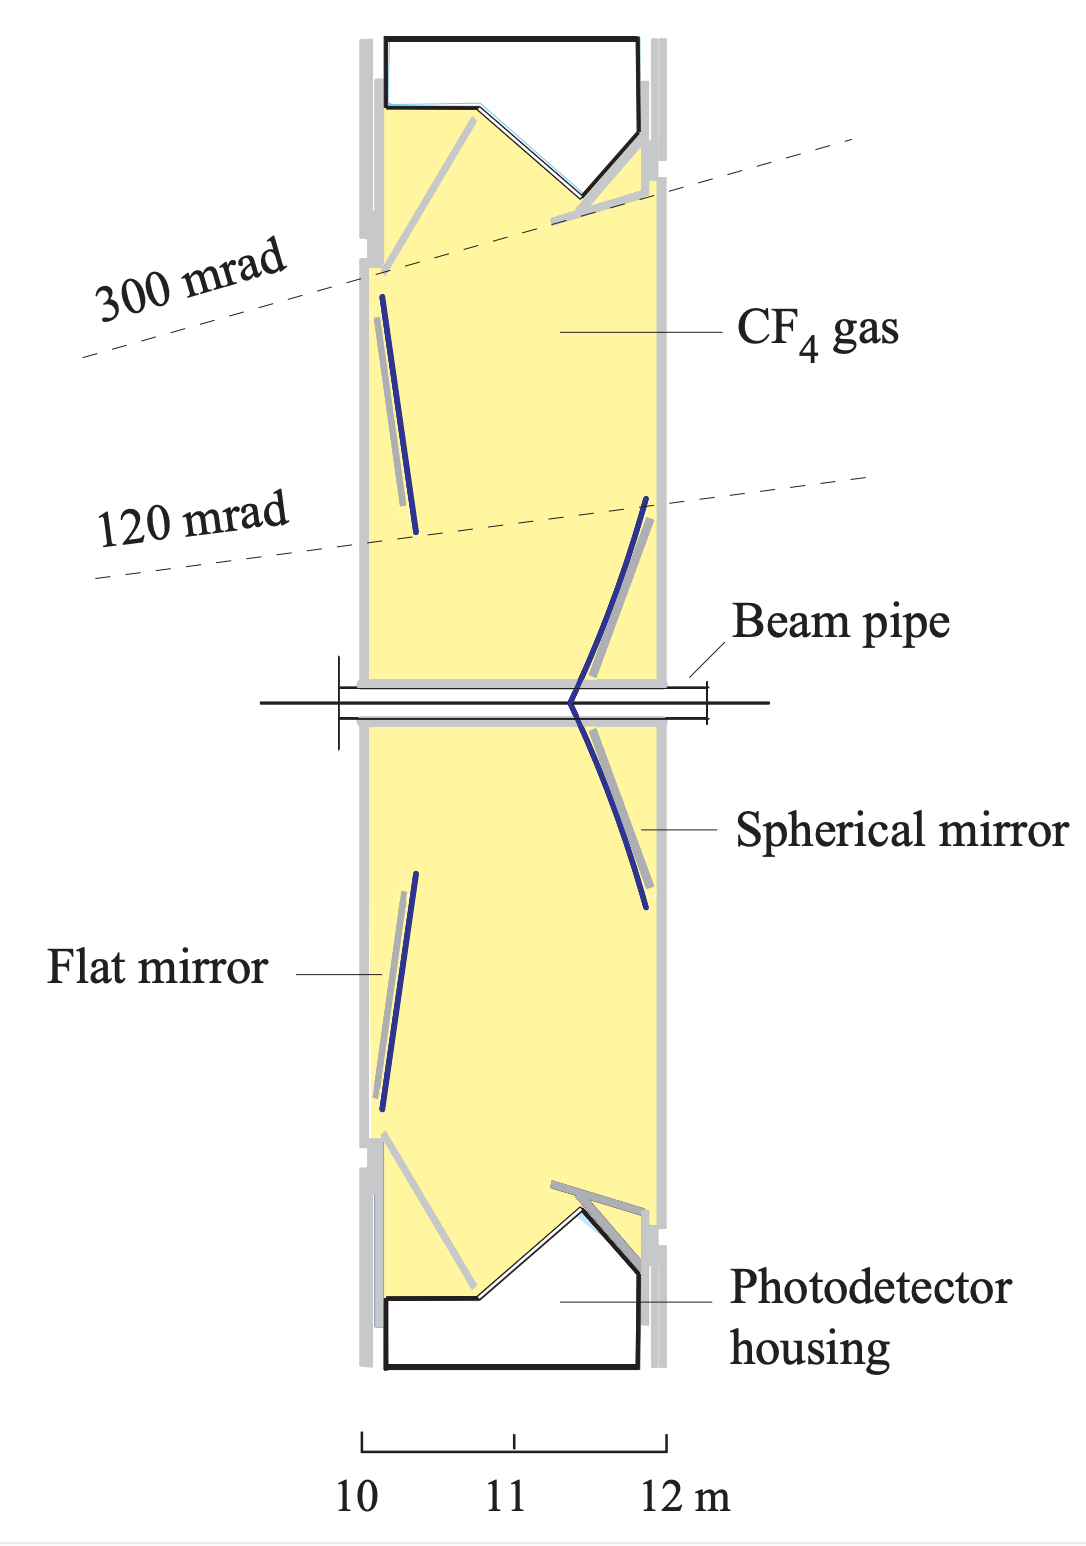
\includegraphics[width=0.4\columnwidth]{figures/detector/RICH2.png}
    \caption{Overview of (left) the RICH 1 and (right) the RICH 2 detectors. Reproduced from Ref.~\cite{LHCb-detector,RICH-TDR}.}
    \label{fig:RICHes}
\end{figure}

Two Ring Imaging CHerenkov detectors (RICH) provide crucial information for particle identification (PID) in \lhcb, in particular the ability to separate pions and kaons that is absolutely essential for the measurement presented in the thesis. The RICH 1 detector is located upstream of the magnet, in between the VELO and the TT tracking station. It is designed to provide PID capability for tracks in the momentum range $p\in[1, 60]\gevc$ using a $\mathrm{C_4F_{10}}$ radiator, and covers the full \lhcb acceptance. During Run~1 the RICH 1 detector also included an Aerogel radiator designed to provide PID for very low momentum particles; however, it was removed before Run~2 because it did not meet the performance requirements during Run~1~\cite{RICH-Performance,RICH-Performance-2}. The RICH 2 detector is located downstream of the T1--T3 tracking stations. It is designed to provide PID capabilities for higher momentum tracks in the range $p\in[15, 100]\gevc$ using a $\mathrm{CF_4}$ radiator. It only covers the very forward region where $|\theta| < 120$\,\mrad ($100$\,mrad) in the horizontal (vertical) directions, as high momentum particles are produced in that region. In both RICH detectors, mirrors are used to reflect the Cherenkov photons to arrays of Hybrid Photon Detectors (HPDs) located outside the \lhcb acceptance. The optics are designed such that photons originating from a given track form rings in the HPD arrays, where the radius is determined by the Cherenkov angle $\theta_c$. The detectors are illustrated in Fig.~\ref{fig:RICHes}.

\begin{figure}[tb]
    \centering
    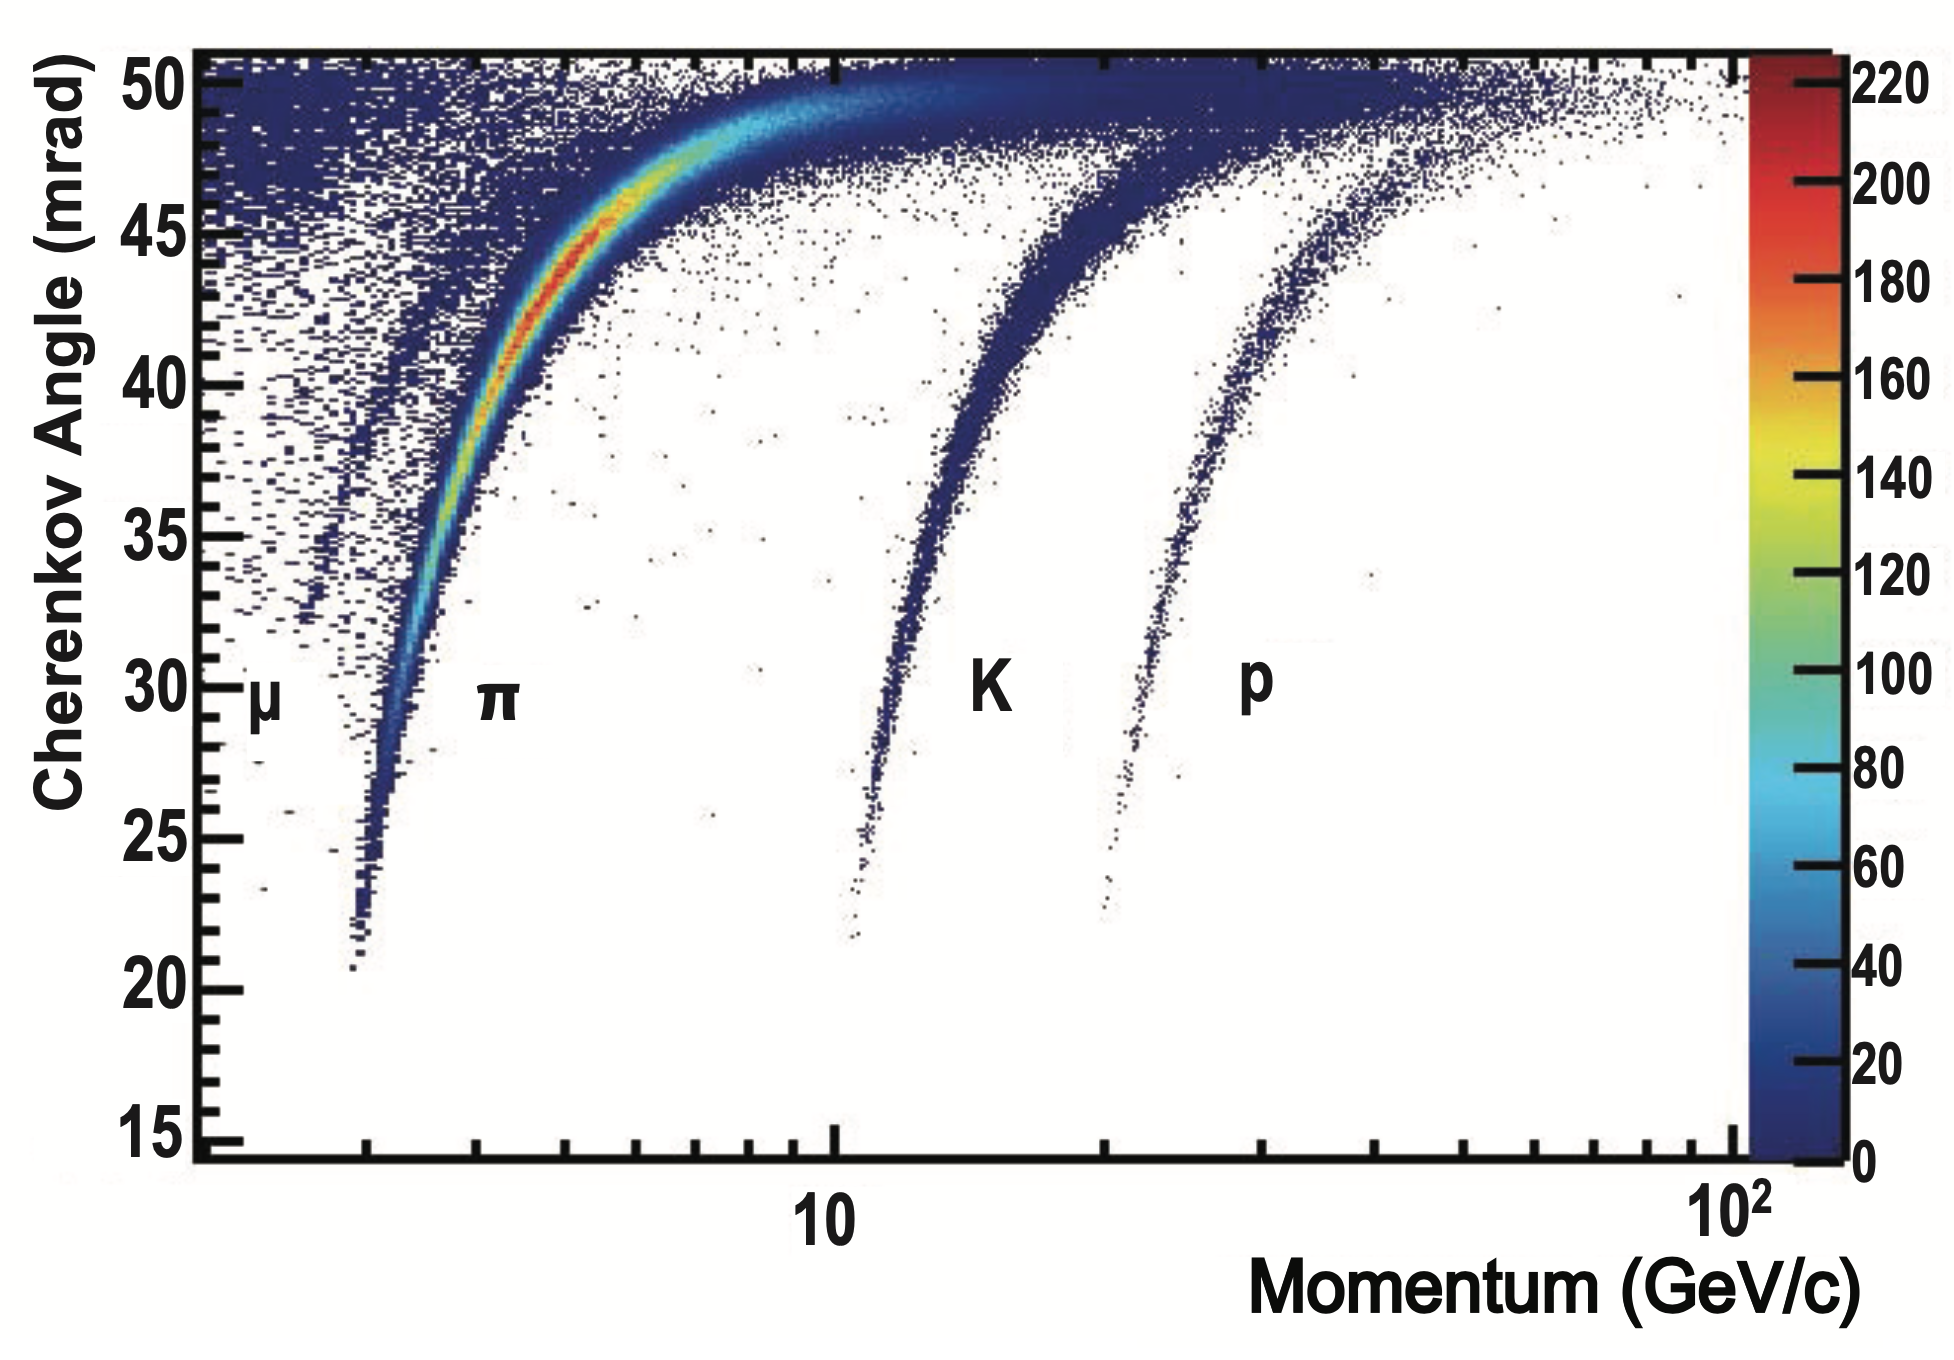
\includegraphics[width=0.55\columnwidth]{figures/detector/RICH_single_track.png}
    \caption{Cherenkov angle for isolated tracks in the RICH 1 radiator as a function of track momentum. Reproduced from Ref.~\cite{RICH-Performance}.}
    \label{fig:RICH_tracks}
\end{figure}

The resolution on $\theta_c$ can be measured by fitting the obtained $\theta_c$ distribution in high momentum tracks, where the Cherenkov angle is saturated. It is found to be $1.618 \pm 0.002$\,mrad for RICH 1 and $0.68 \pm 0.02$\,mrad for RICH 2 in Run~1 data~\cite{RICH-Performance}, and was essentially unchanged in Run~2~\cite{RICH-Performance-2}. Figure~\ref{fig:RICH_tracks} shows the relation between track momentum and $\theta_c$ in RICH 1 for \emph{isolated tracks} in Run~1 data; these are tracks where the Cherenkov ring does not overlap with any other Cherenkov rings. The bands for each hadron species are clearly visible, and it can be seen that the RICH detector also provide some ability to distinguish muons. The definition of the PID variables used in analysis is discussed in Section~\ref{sub:particle_identification}, along with the achieved PID performance.
% subsection the_rich (end)

\subsection{Calorimeters} % (fold)
\label{sub:calorimeters}

The calorimeter system of the \lhcb detector has four components. Ordered from the interaction point, these are the Scintillating Pad Detector (SPD), the Pre-Shower (PS) detector, an Electromagnetic Calorimeter (ECAL), and a Hadron Calorimeter (HCAL). In all four cases, light is produced in organic scintillators and transmitted to Photo Multiplier Tubes (PMTs) via optical fibres~\cite{LHCb-detector}. Information from the calorimeters provide identification of electrons, photons, and hadrons, and measurements of their energies and positions, and also plays a crucial role in the triggering, as described below. 

\begin{figure}[tb]
    \centering
    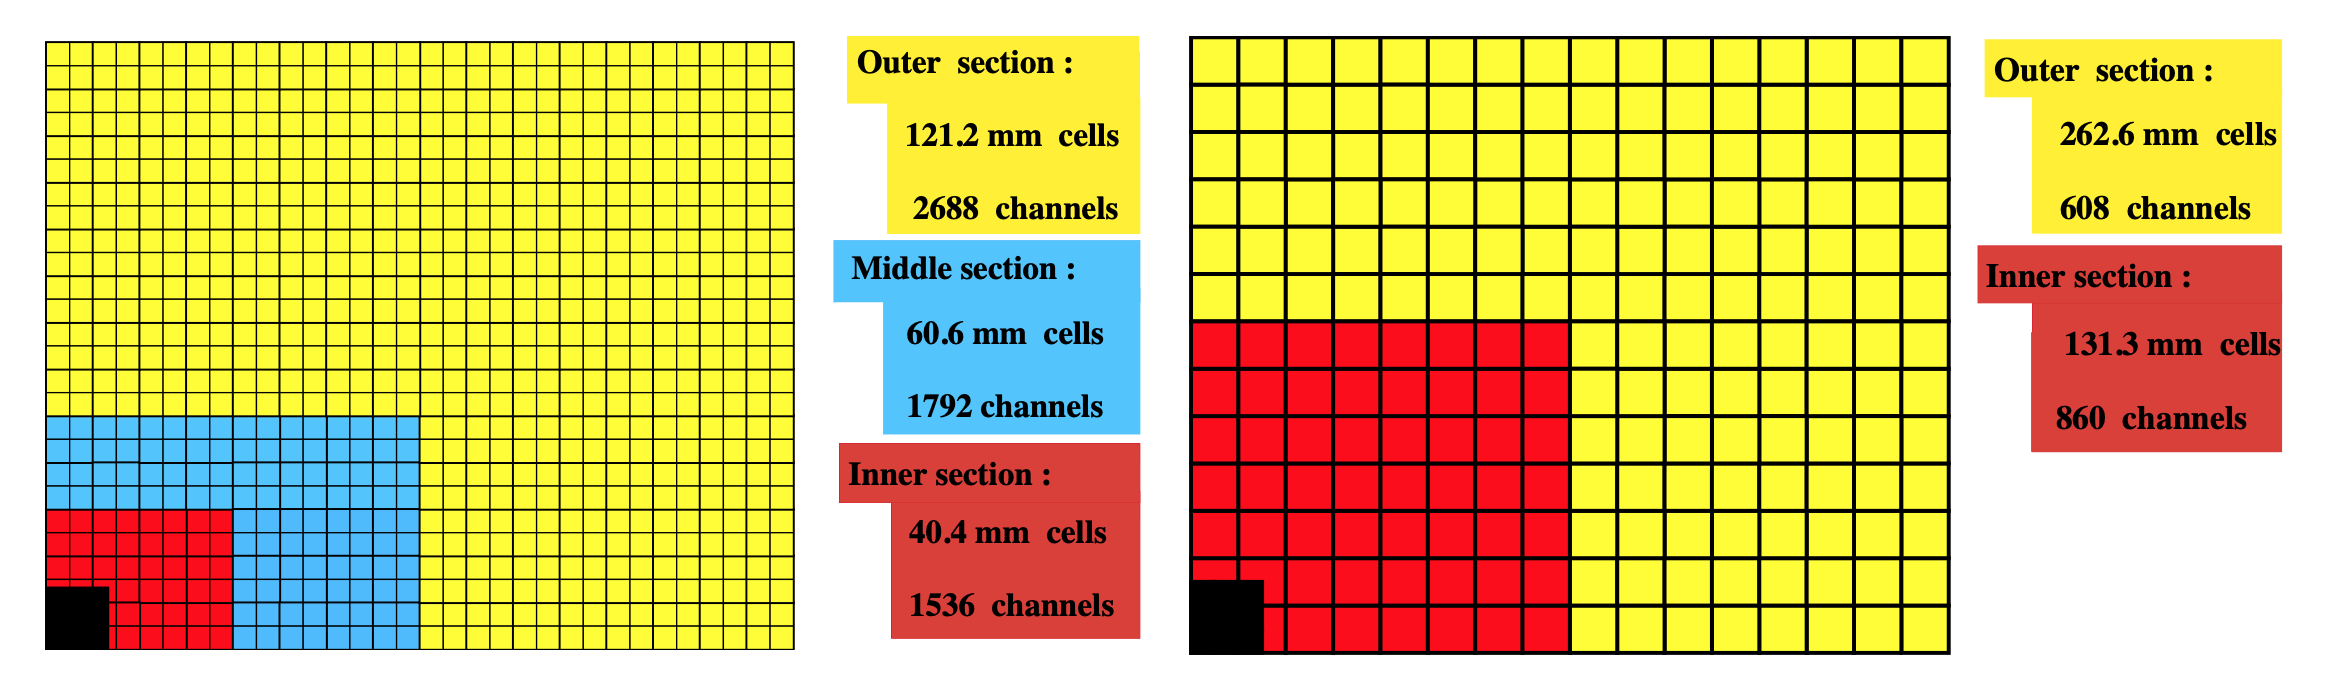
\includegraphics[width=0.9\columnwidth]{figures/detector/cell_modules.png}
    \caption{Illustration of the calorimeter cell size of (left) the ECAL and (right) the HCAL. Reproduced from Ref.~\cite{CAL-TDR}.}
    \label{fig:cal_cells}
\end{figure}

The SPD and PS detectors consist of almost identical planes of rectangular scintillator pads, with a 15\mm thick lead absorber located in between. The presence of the SPD before the first absorption layer allows for the separation of photons and electrons in the trigger, because only electrons cause a signal in the SPD. The PS allows for the separation of pion and electron tracks, as only the latter interacts significantly with the thin layer of lead. The cell divisions of the detectors closely follow that of the ECAL, shown in Fig.~\ref{fig:cal_cells}, to allow for the matching of energy deposits.

\begin{figure}[tb]
    \centering
    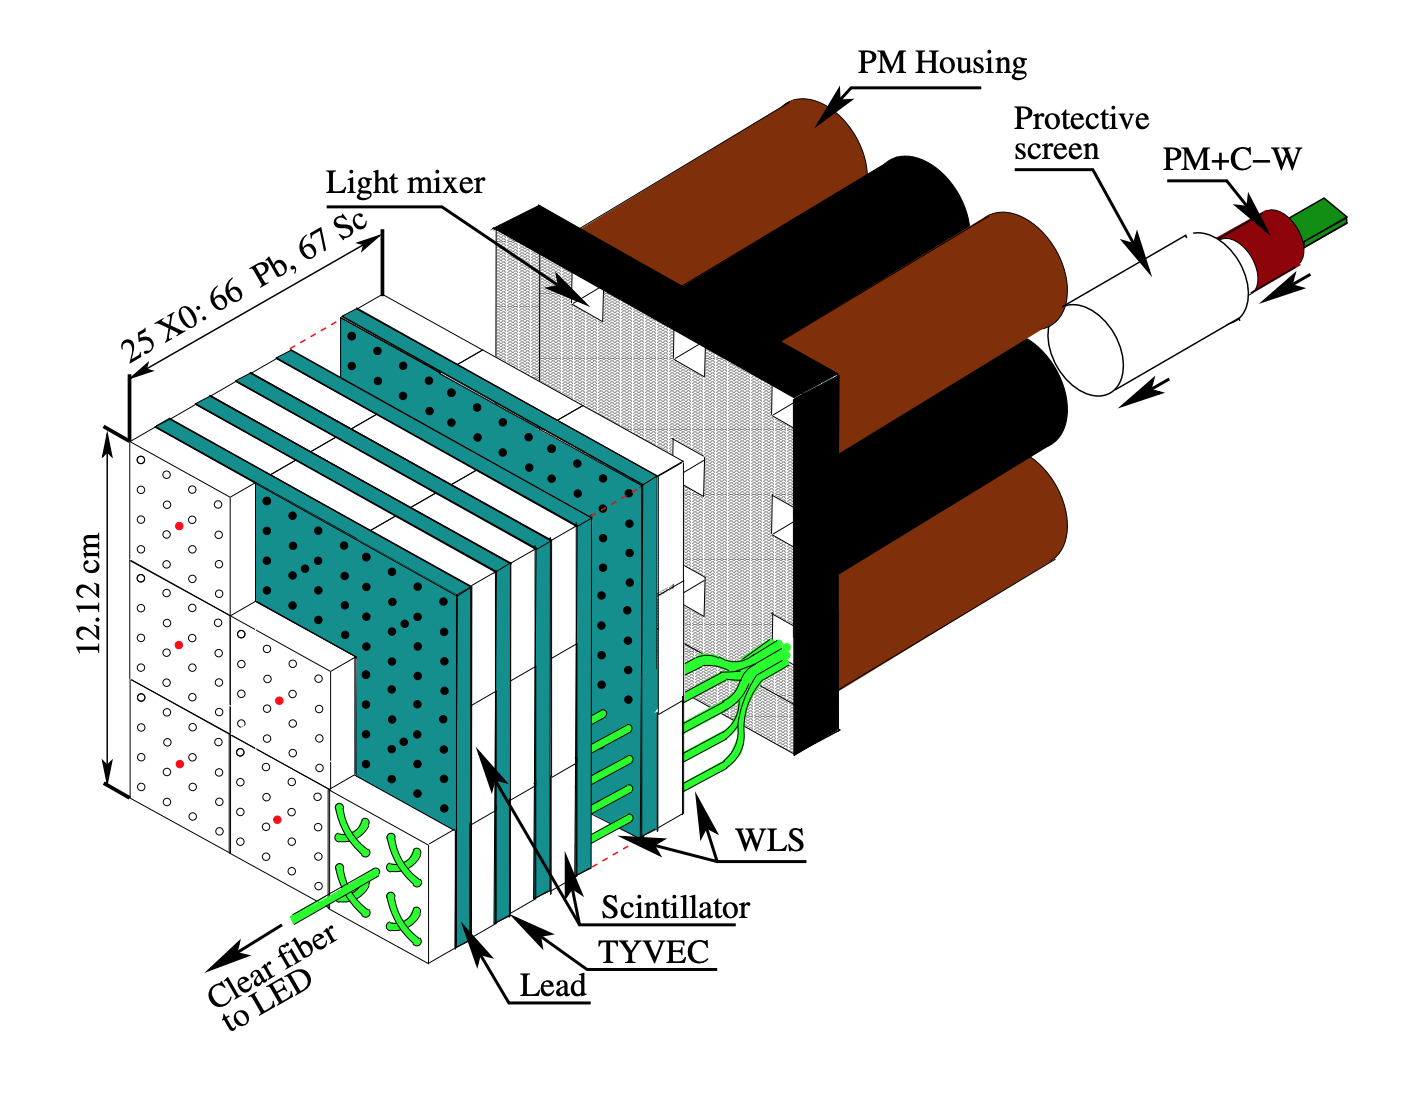
\includegraphics[width=0.55\columnwidth]{figures/detector/ECAL_module.png}
    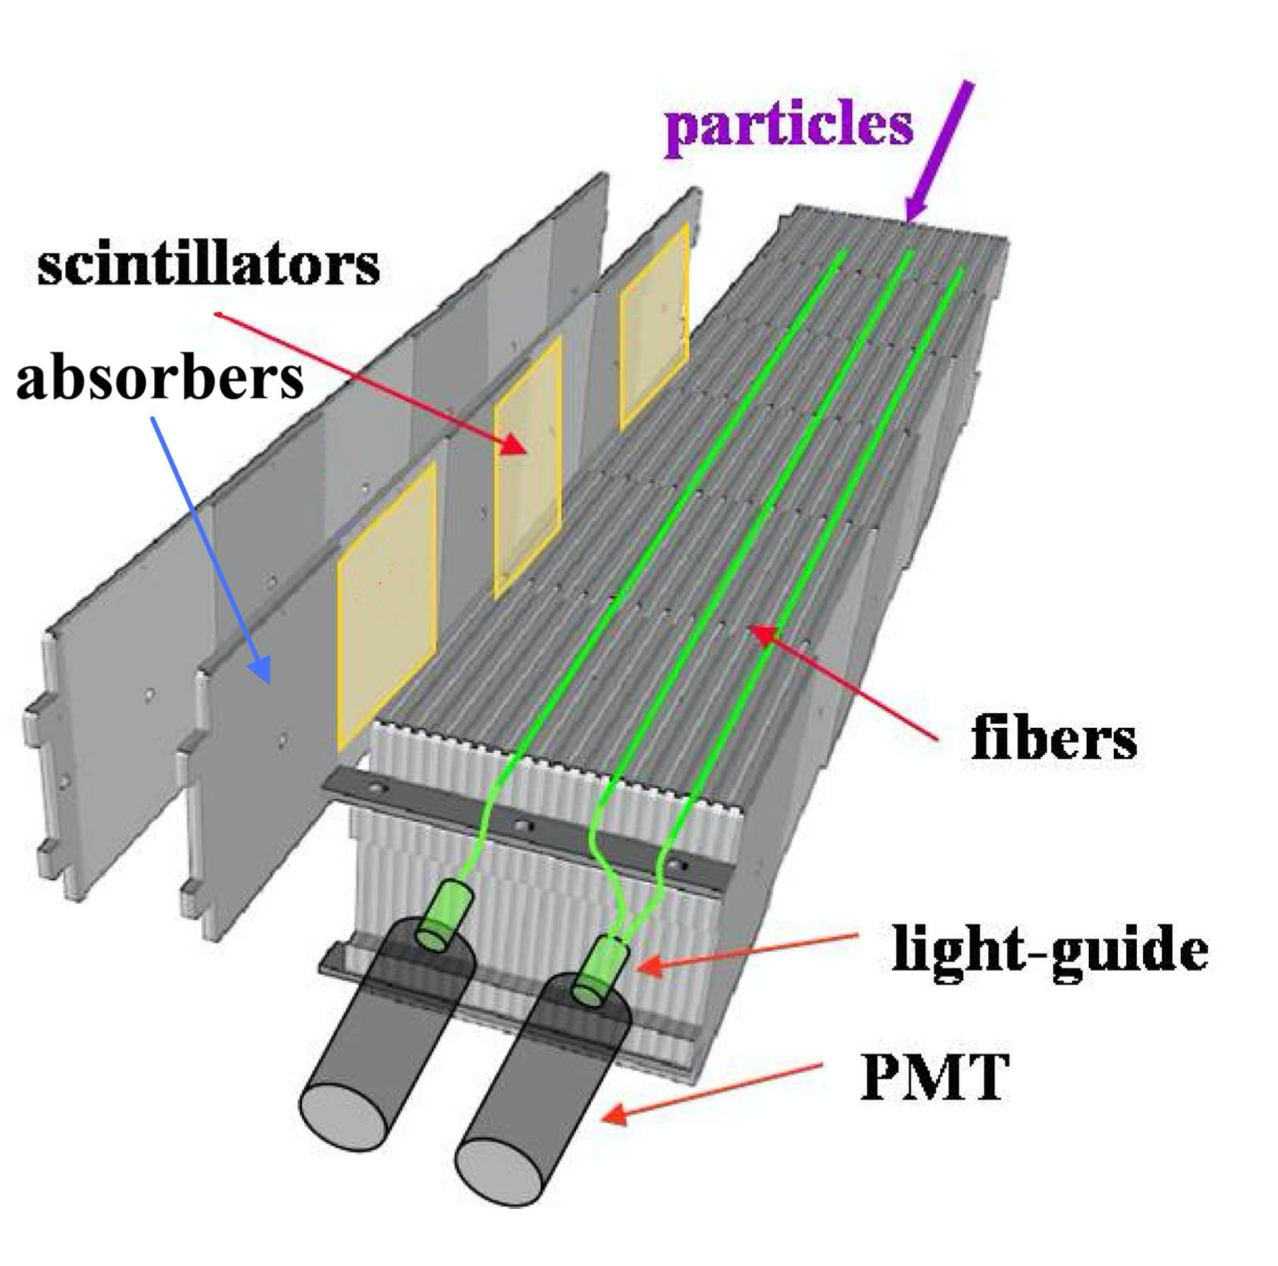
\includegraphics[width=0.40\columnwidth]{figures/detector/HCAL_module.png}
    \caption{Illustration of (left) an ECAL and (right) an HCAL module. Reproduced from Refs.~\cite{ECALpaper,LHCb-Performance}.}
    \label{fig:ECAL_HCAL_modules}
\end{figure}

The ECAL has a Shashlik structure, with 66 layers consisting of 2\mm of lead absorber and 4\mm of scintillator; an example of a calorimeter module is shown in Fig.~\ref{fig:ECAL_HCAL_modules}. Accurate energy measurements require that the full electronic shower is contained in the ECAL, which is achieved since the structure extends for 25 radiation lengths. The scintillators are divided into cells that allow for the determination of the location and shape of energy deposits; the cell dimensions vary as a function of radial distance from the beam pipe as shown in Fig.~\ref{fig:cal_cells}, to take into account the varying occupancy. The resolution of the ECAL has been measured to be $\Delta E/E \simeq (9/\sqrt{E} \bigoplus 0.8)\,\%$ ($E$ in \gevcc)~\cite{LHCb-detector}.

The HCAL is located downstream of the ECAL, designed to measure the energy of hadrons (which leave relatively little energy in the ECAL). It is constructed with layers of 1\cm iron absorbers inter-spaced with scintillators, oriented \emph{along} the beam direction, such that a typical track will traverse 16\mm of iron per 4\mm of scintillator~\cite{CAL-TDR}. As for the ECAL, the cell size varies as a function of distance to the beam line, as shown in Fig.~\ref{fig:cal_cells}. An example of a module is shown in Fig.~\ref{fig:ECAL_HCAL_modules}.  The energy resolution required for efficient triggering is moderate; therefore,  the HCAL only has a length of 5.6 interaction lenghts and can measure the hadron energies at a resolution of $\Delta E/E \simeq (69/\sqrt{E} \bigoplus 9)\,\%$ ($E$ in \gevcc)~\cite{LHCb-detector}.

% subsection calorimeters (end)

\subsection{Muon detectors} % (fold)
\label{sub:muon_detectors}

\begin{figure}[tb]
    \centering
\begin{subfigure}{0.45\columnwidth}
    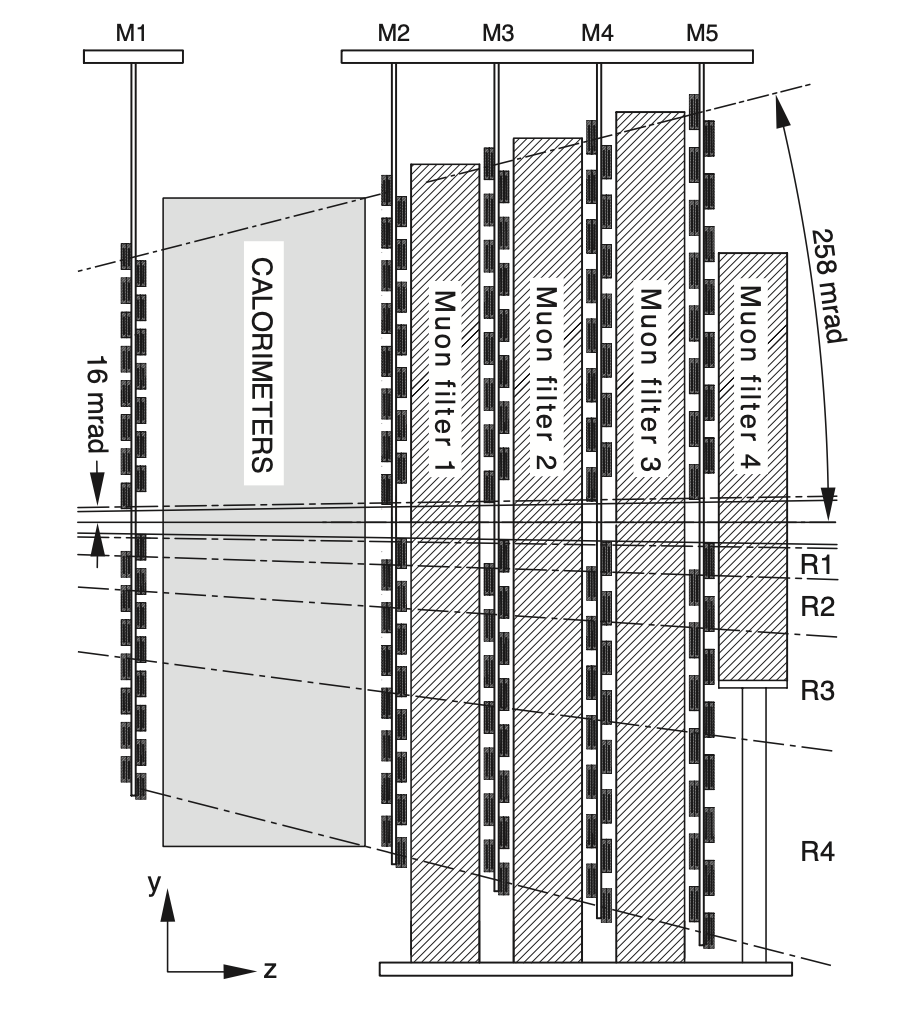
\includegraphics[width=\columnwidth]{figures/detector/muon_stations.png}
    \caption{}
    \label{fig:muon_stations}
\end{subfigure}
\begin{subfigure}{0.45\columnwidth}
    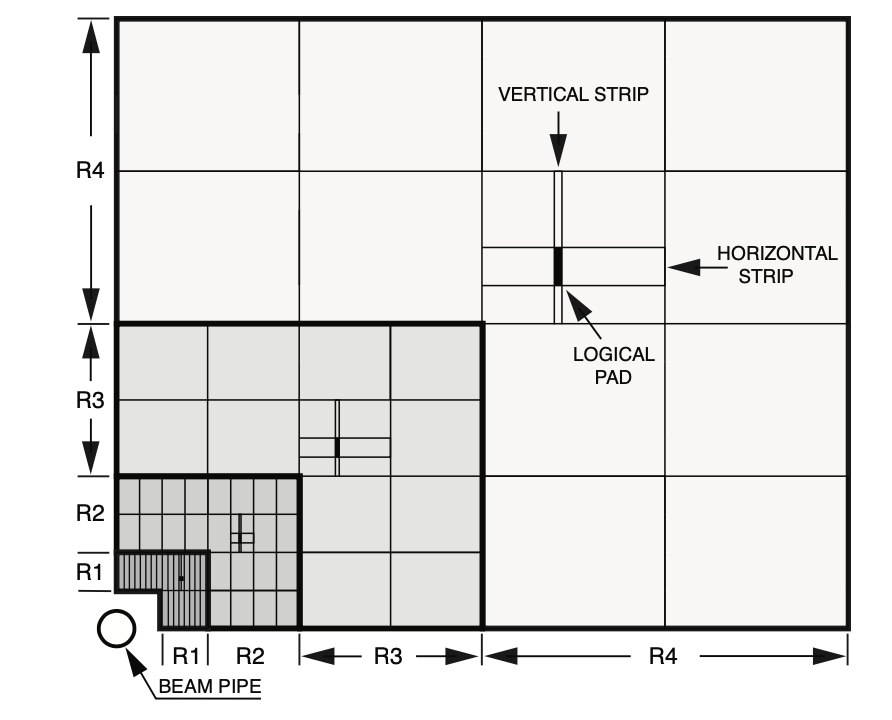
\includegraphics[width=\columnwidth]{figures/detector/muon_pad.png}
    \caption{}
    \label{fig:muon_pad}
\end{subfigure}
    \caption{Illustration of (a) the location of the muon stations along the $z$-axis of the experiment and (b) the geometry of the logical pads of the M3 muon station. Reproduced from Ref.~\cite{LHCb-Performance}.}
\end{figure}

Muon identification and triggering is crucial for a range of high-profile \lhcb measurements, such as lepton-universality tests~\cite{LHCb-PAPER-2019-009,LHCb-PAPER-2020-002} or measurements of  $B^0_{(s)}\to\mup \mu^-$ decays~\cite{LHCb-PAPER-2017-001}. In the thesis, muon identification plays a role in suppressing a number of backgrounds. The \lhcb muon system consists of 5 tracking stations, M1--M5, covering the full \lhcb acceptance. M1 is located upstream of the ECAL, whereas M2--M5 are located downstream of the HCAL and inter-spaced with 80\cm thick iron absorbers in order to select penetrating muons. This is illustrated in Fig.~\ref{fig:muon_stations}. The detectors are predominantly multiwire proportional chambers (MWPC), organised into logical pads, the dimensions of which define the $(x, y)$ resolution of the measured spatial points. The exception is the central region of the M1 station, which is a triple gas-electron-multiplier detector, due to the higher track density in that region~\cite{LHCb-TDR-5-add-2}. As for the calorimeters, the size of the pads vary as a function of the radial distance from the beam pipe, as illustrated in Fig.~\ref{fig:muon_pad}. The resolution is significantly better in the bending plane ($x$) than in the non-bending plane ($y$). The resolution is also significantly better in the M1--3 stations than in M4 and M5, which are mostly used to identify penetrating tracks. The muon system can independently measure the $p_T$ of a muon to within 20\,\%, which allows for efficient triggering.

% subsection muon_detectors (end)

% section subdetectors (end)

\section{Reconstruction} % (fold)
\label{sec:reconstruction}

This section describes the reconstruction algorithms that fit detector hits in the tracking stations to form track candidates, as well as the algorithms used to identify the types of the particles that formed these tracks.

% section reconstruction (end)

\subsection{Track reconstruction} % (fold)
\label{sub:track_reconstruction}

\begin{figure}[tb]
    \centering
    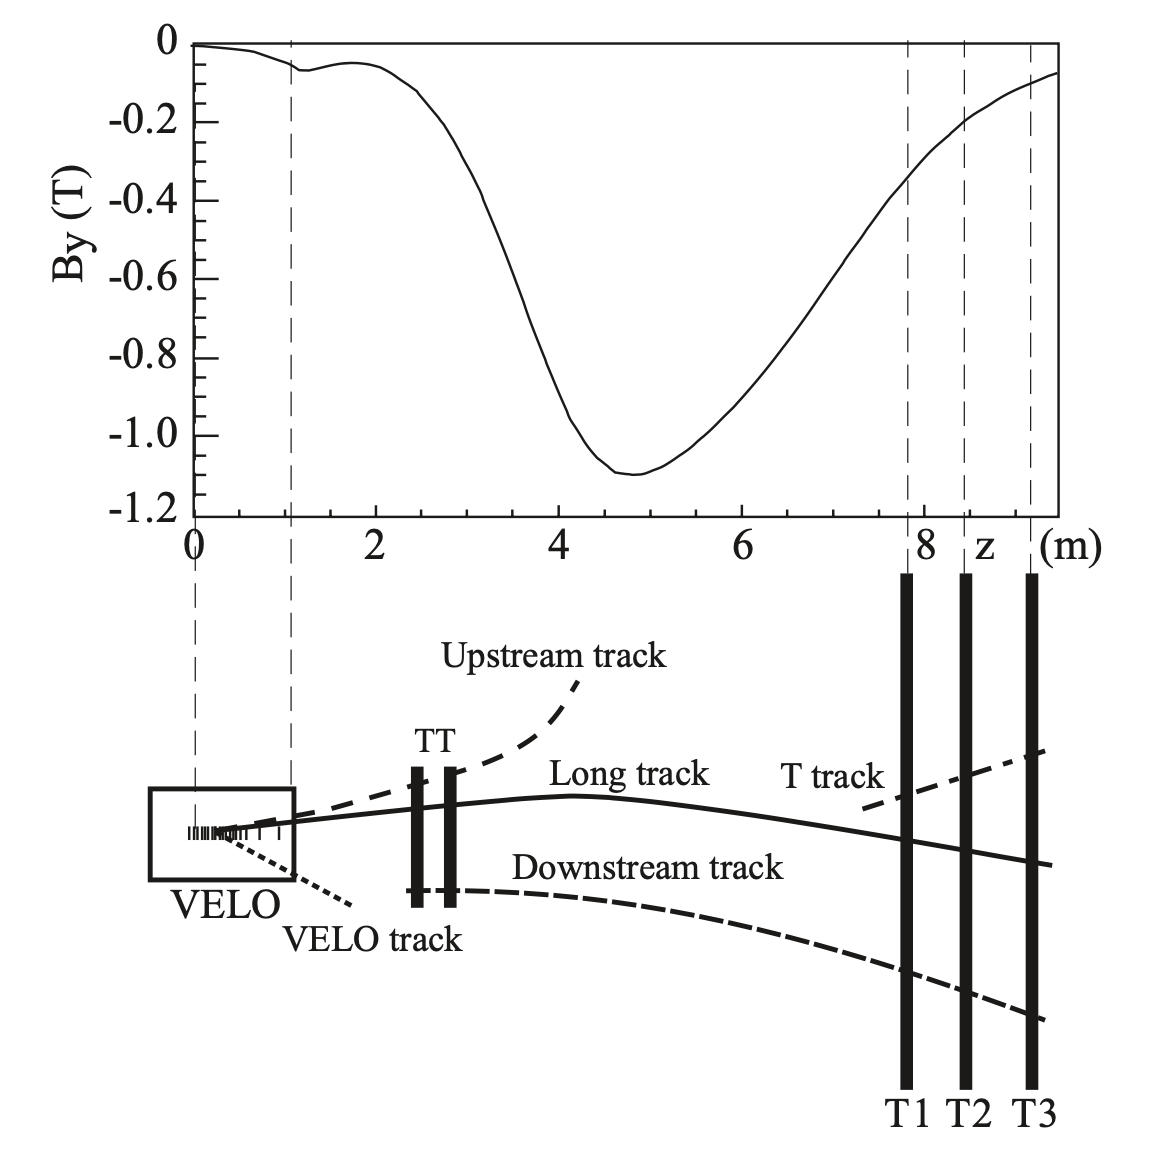
\includegraphics[width=0.75\columnwidth]{figures/detector/track_types.png}
    \caption{Definition of track types within the \lhcb detector, depending on which set of tracking detectors the track intersects. The profile of the magnetic field  is also shown. Reproduced from Ref.~\cite{LHCb-Performance}.}
    \label{fig:track_types}
\end{figure}

The \lhcb experiments operates with a number of different particle track types, depending on which sub detectors a track intersects; these are summarised in Fig.~\ref{fig:track_types}. The two track types that are important for this thesis are \emph{long} tracks, which have hits in the VELO and the TT and T1--T3 tracking stations, and \emph{downstream} tracks that only have hits in the TT and T1--3 tracking stations. The analysis depends on both track types because a number of \KS mesons produced in the signal decay leave the VELO before they decay into the $\pip\pim$ final state that is reconstructed; hence these pions necessarily form downstream tracks.

The first step is to form track candidates from hits in the VELO (VELO tracks) and T1--3 stations (T tracks) separately; because the magnetic field is low in the tracking detectors, these tracks are fairly straight. Long tracks are formed using two separate search strategies: in one, \emph{forward tracking}~\cite{VELO-Forward}, VELO tracks are used as seeds and matched with hits in the TT and T1--3 tracking stations by extrapolation. These are combined to form long tracks that are required to pass a set of quality conditions. An alternative approach, \emph{track matching}~\cite{VELO-Match,VELO-Match2}, matches VELO and T tracks by extrapolating both through the bending region, and deciding if they below together; finally TT hits are added. The union of tracks found via both approaches is saved, where only the track candidate with the best fit quality is kept in the case where a track appears twice. Downstream tracks are formed based on T tracks as seeds, matched with hits in the TT detector in a search region obtained by extrapolation of the seed~\cite{Downstream}. Finally, each track is reprocessed using a Kalman filter that takes into account multiple scattering and corrects for energy loss due to ionisation~\cite{fruhwirthApplicationKalmanFiltering1987,VanTilburg:885750}.

\begin{figure}[tb]
    \centering
    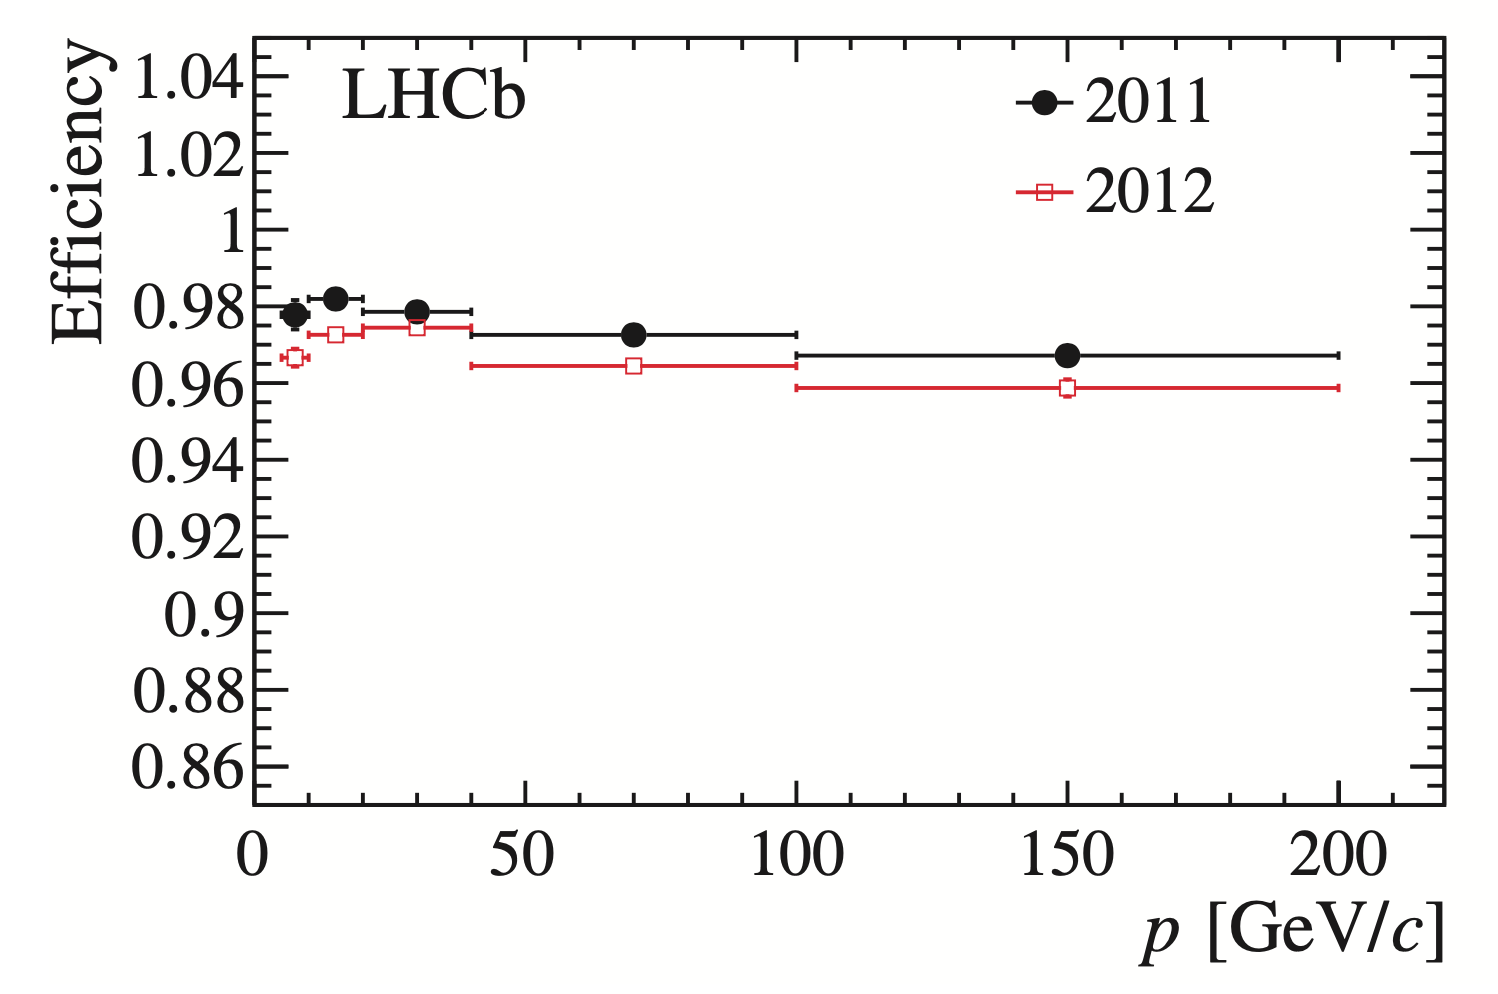
\includegraphics[width=0.45\columnwidth]{figures/detector/track_eff_p.png}
    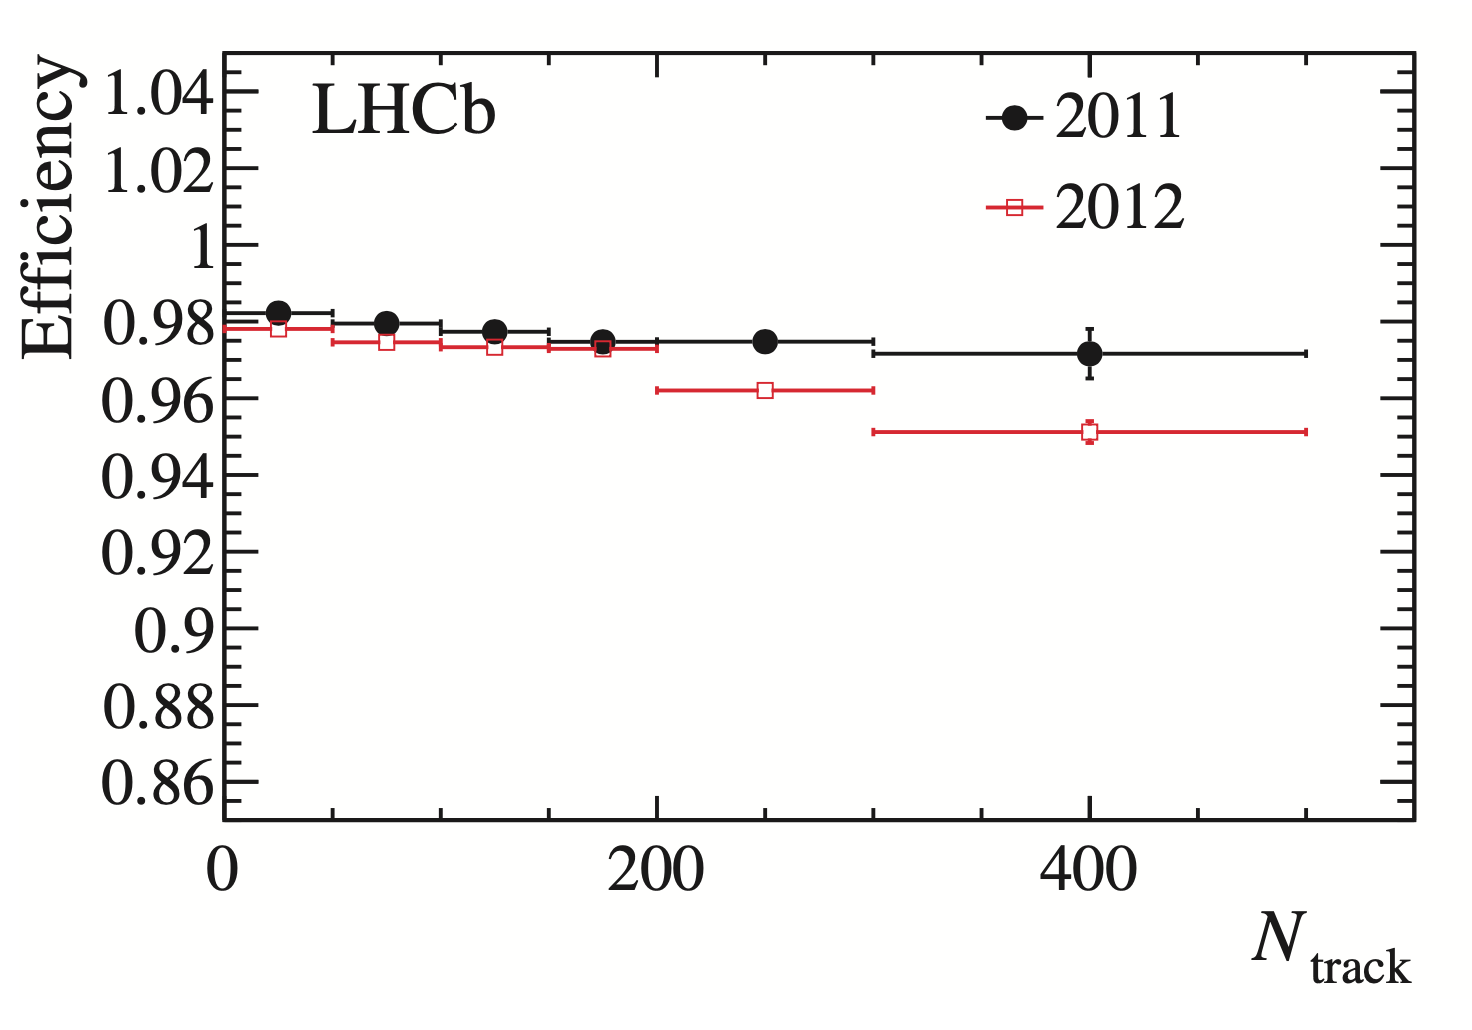
\includegraphics[width=0.45\columnwidth]{figures/detector/track_eff_N.png}
    \caption{The long track reconstruction efficiency as a function of (left) track momentum and (right) the number of charged tracks in the event. The lower efficiency in 2012 than 2011 is partially due to the higher event multiplicity, given the higher centre-of-mass energy. The figure is reproduced from Ref.~\cite{LHCb-Performance}.}
    \label{fig:track_eff}
\end{figure}

Many of the interesting signal decay channels of \lhcb have 4--6 charged final state tracks, and therefore it is crucial to have a single-track reconstruction efficiency close to 100\,\%. The single-track reconstruction efficiency is shown in Fig.~\ref{fig:track_eff} as a function of track momentum and the number of tracks in an \emph{event} (an \emph{event} denotes a $pp$ collision and all the particles produced therein and in subsequent decays). The efficiencies have been obtained in data, using a tag-and-probe method in $J/\psi\to\mup\mu^-$ decays~\cite{TrackEff}. One muon, the \emph{tag}, is fully reconstructed, while the other, the \emph{probe} is only partially reconstructed, allowing for the $J/\psi$ invariant mass to be reconstructed with reasonable resolution. If the partially reconstructed probe track is matched to a full long track, the track is classified as efficient.
Similar efficiencies have been achieved in Run~2.




\subsection{Particle identification} % (fold)
\label{sub:particle_identification}
The information from the RICH detectors, the calorimeters, and the muon system is combined for optimal identification of charged tracks as electrons, muons, pions, kaons, or protons. Photons and neutral pions are identified using the ECAL, but play no role in the thesis, and will not be discussed further.

\begin{figure}[tb]
    \centering
    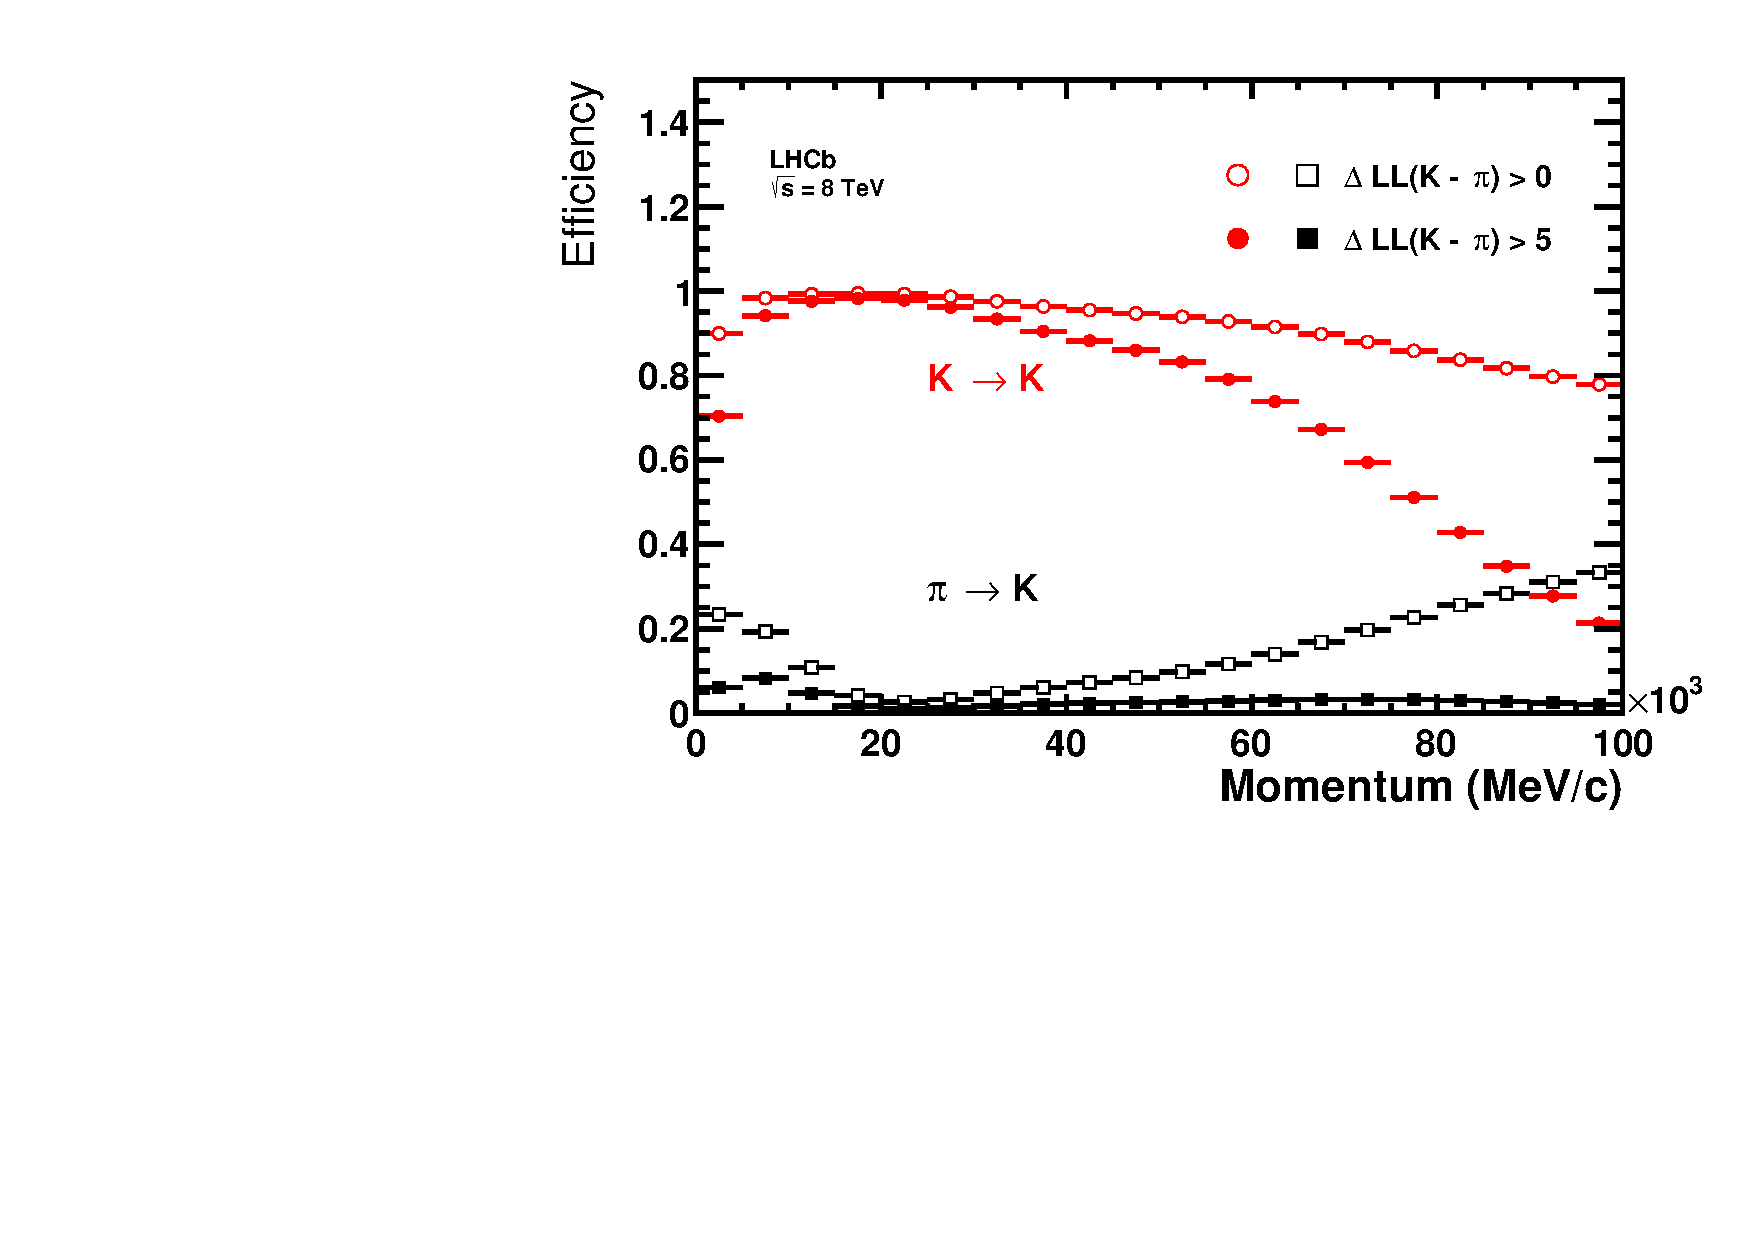
\includegraphics[width=0.45\columnwidth]{figures/detector/PIDK_Run1.pdf}
    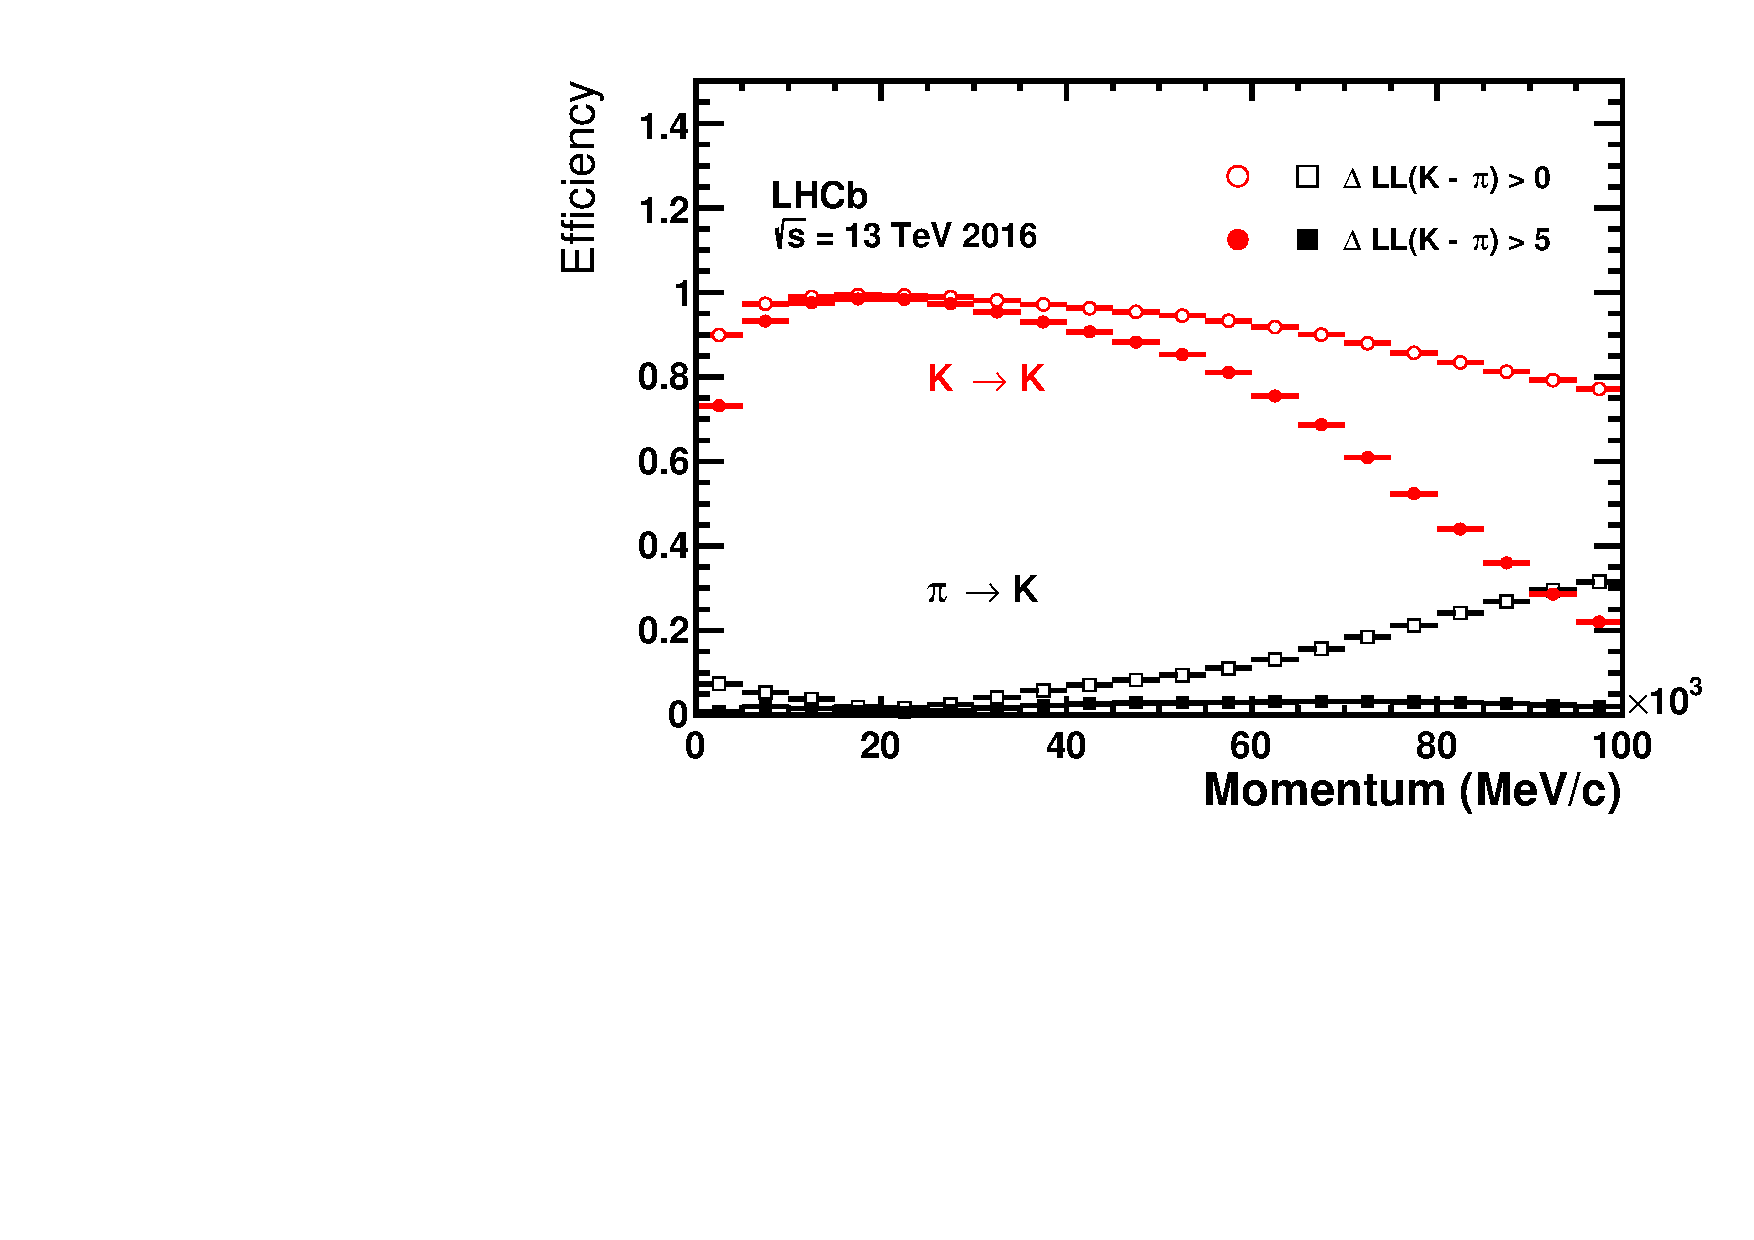
\includegraphics[width=0.45\columnwidth]{figures/detector/PIDK_Run2.pdf}
    \caption{The probability to correctly identify a kaon/misidentify a pion as a kaon given two different requirements on $\Delta \mathrm{LL}(K-\pi)$, as a function of track momentum in (left) Run~1 data from 2012 and (right) Run~2 data from 2016. Reproduced from Ref.~\cite{PIDplots}.}
    \label{fig:PID_performance}
\end{figure}

The ability to separate \BtoDK and \BtoDpi decays is essential to the measurement presented in this thesis. In \lhcb, hadron separation is achieved via information from the RICH detectors, using a likelihood method where the observed pattern of hit pixels in the photo detectors is compared to the expected pattern, given all reconstructed tracks in an event under a given set of particle hypothesis. The likelihood is maximised by varying the particle hypotheses for each track being an electron, muon, pion, kaon, or proton~\cite{Forty:684714}.  It is necessary to consider all tracks of an event simultaneously because the Cherenkov rings of different tracks overlap. For each track, the maximum log likelihood of a particle hypothesis, say that the track is a kaon, relative to the hypothesis that it is a pion
\begin{align}\label{eq:DLL}
    \Delta\text{LL}_{\text{track}_i}^\text{RICH}(K-\pi) =  \ln \mathcal L_\text{max}^\text{RICH}(\text{pattern}|\text{track}_i = K)\ - \ln \mathcal L_\text{max}^\text{RICH}(\text{pattern}|\text{track}_i = \pi),
\end{align}
is saved to inform PID decisions. In the case of pion-kaon separation, this variable alone is enough to achieve good separation power; in the remainder of the thesis it is denoted \texttt{PIDK}. The PID performance for pion-kaon separation has been measured in calibration data, following a procedure described in Section~\ref{sub:efficiency_of_the_pid_requirements}, and is illustrated in Fig.~\ref{fig:PID_performance}.

\begin{figure}[tb]
    \centering
    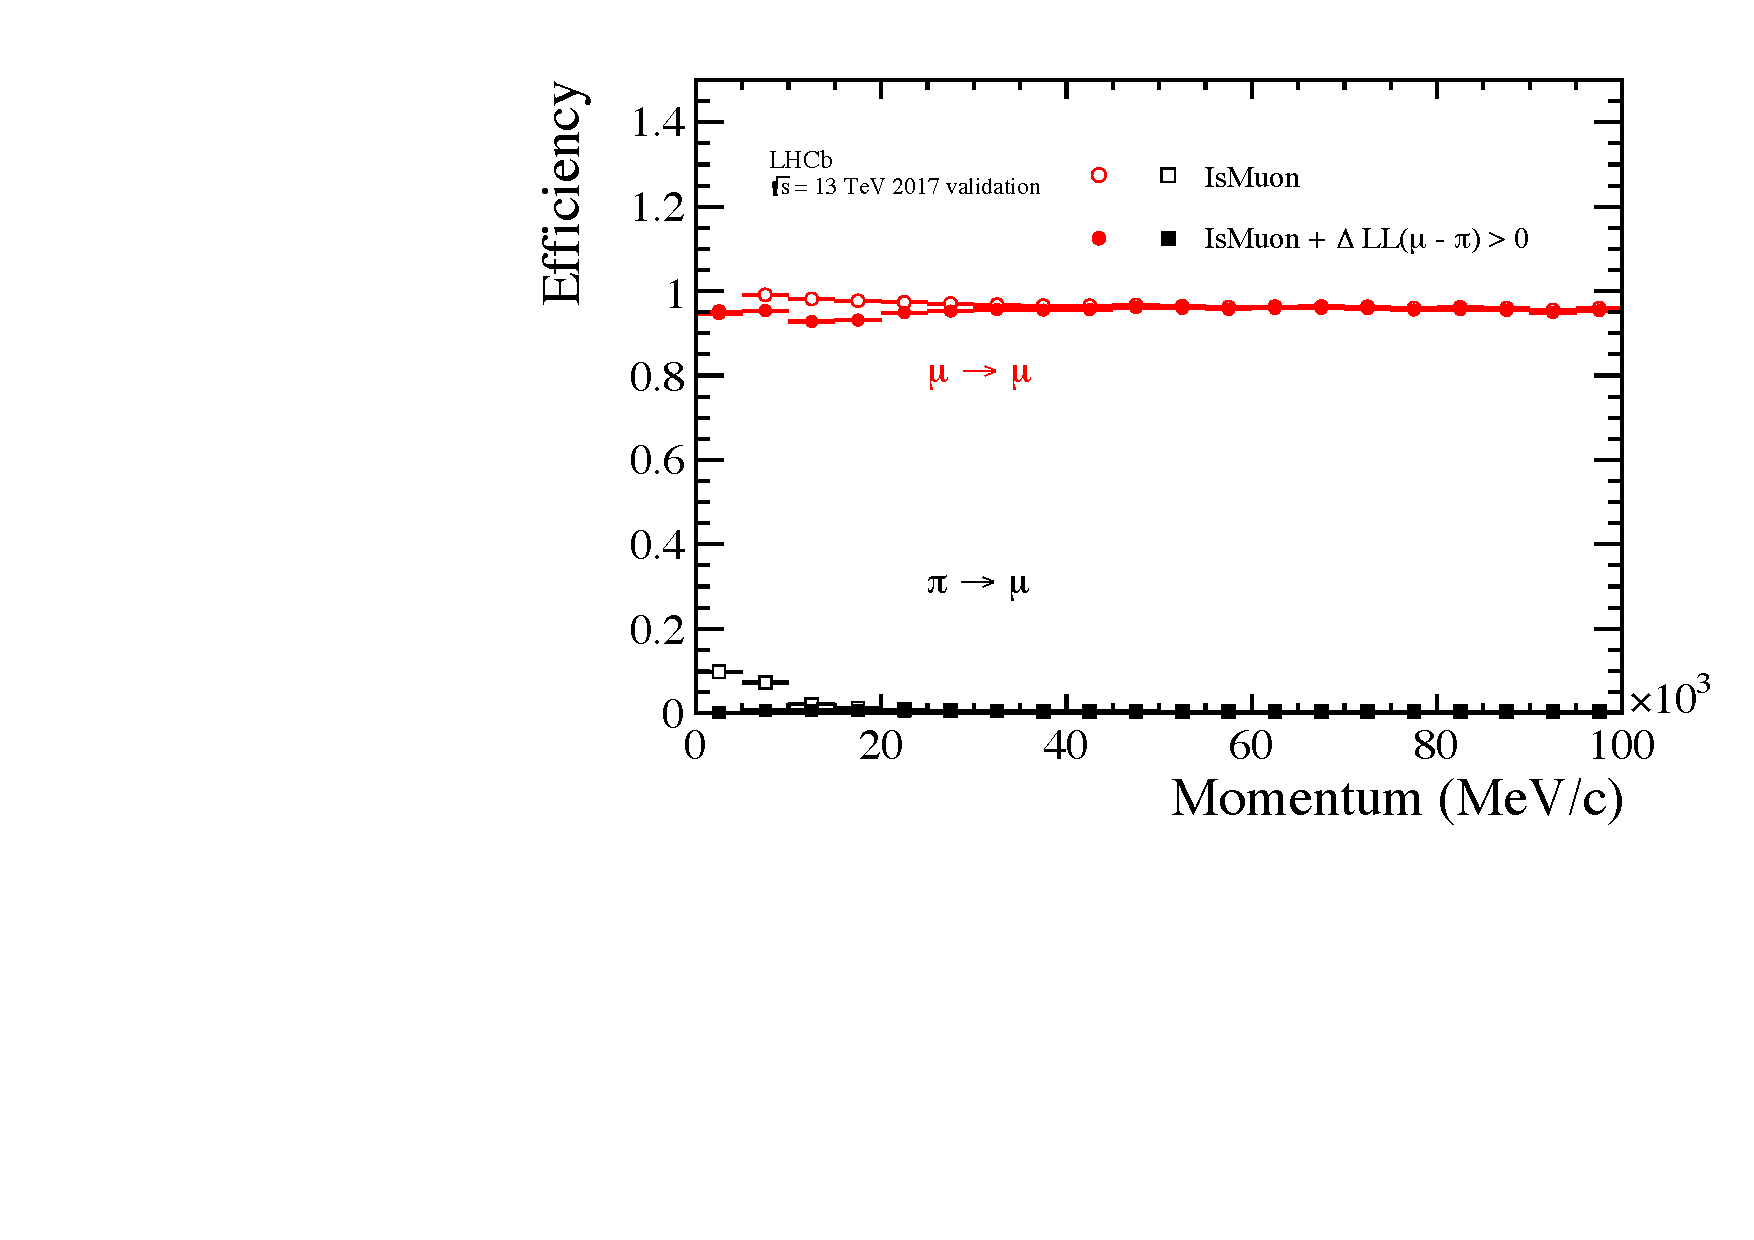
\includegraphics[width=0.60\columnwidth]{figures/detector/PIDmu_Run2.pdf}
    \caption{The probability to correctly identify a muon/misidentify a pion as a muon given requirements on either \texttt{isMuon} or $\Delta \mathrm{LL}(\mu-\pi)$, as a function of track momentum in Run~2 data from 2017. Reproduced from Ref.~\cite{PIDplots}.}
    \label{fig:PIDmu_performance}
\end{figure}

Muons are identified by extrapolating tracks to the muon stations to define fields-of-interest (FOI). A track is considered as a muon candidate when a minimum number of stations (2--4 depending on the track momentum) have hits in the corresponding FOI~\cite{MuonPID,MuonPID2}. This information is encoded in a variable denoted \texttt{isMuon} throughout the thesis. Additional information, such as a comparison of the slopes of the track in the main tracker and the muon stations, and the average track-hit distance in the FOI is used to form a $\Delta \text{LL}^\text{muon}(\mu-\pi)$ variable analogous to the one defined in Eq.~\eqref{eq:DLL} for the RICH detectors; again defining as the relative likelihood with respect to the pion hypothesis. This variable can be combined with $\Delta \text{LL}^\text{RICH}(\mu-\pi)$ to form a $\Delta \text{LL}(\mu-\pi)$ variable that takes information from both detectors into account, denoted \texttt{PIDmu}. The performance of the muon PID variables is shown in Fig.~\ref{fig:PIDmu_performance} as obtained in data. It can be seen that requiring $\texttt{isMuon=0}$ rejects muon tracks efficiently at all momenta; this is used in the analysis to veto a number of semi-leptonic backgrounds.

In similar manner, a potential semi-leptonic background with electrons is also vetoed in the analysis presented in the thesis. In \lhcb, electron PID is mainly based on the balance between deposited energy and track momentum in the ECAL~\cite{ElectronPID}. This information is combined with information on photon energy deposits from brehmstrahlung, and energy deposits in the PS and HCAL, as well as information from the RICH and muon detectors, to form yet another $\Delta\text{LL}(e-\pi)$ variable as the likelihood difference between the electron and pion hypotheses, denoted \texttt{PIDe}. As an example of the obtainable performance, an average electron selection effiency of $(91.9\pm1.3$\,\% was achieved in displaced $J/\psi\to e^+e^-$ decays in Run~1, with a hadron misidentification rate of $(5.54\pm0.02)$\,\%~\cite{LHCb-Performance}.

% subsection particle_identification (end)

% section reconstruction (end)

\section{The LHCb trigger system} % (fold)
\label{sec:the_lhcb_triggerring_system}

\begin{figure}[tb]
    \centering
    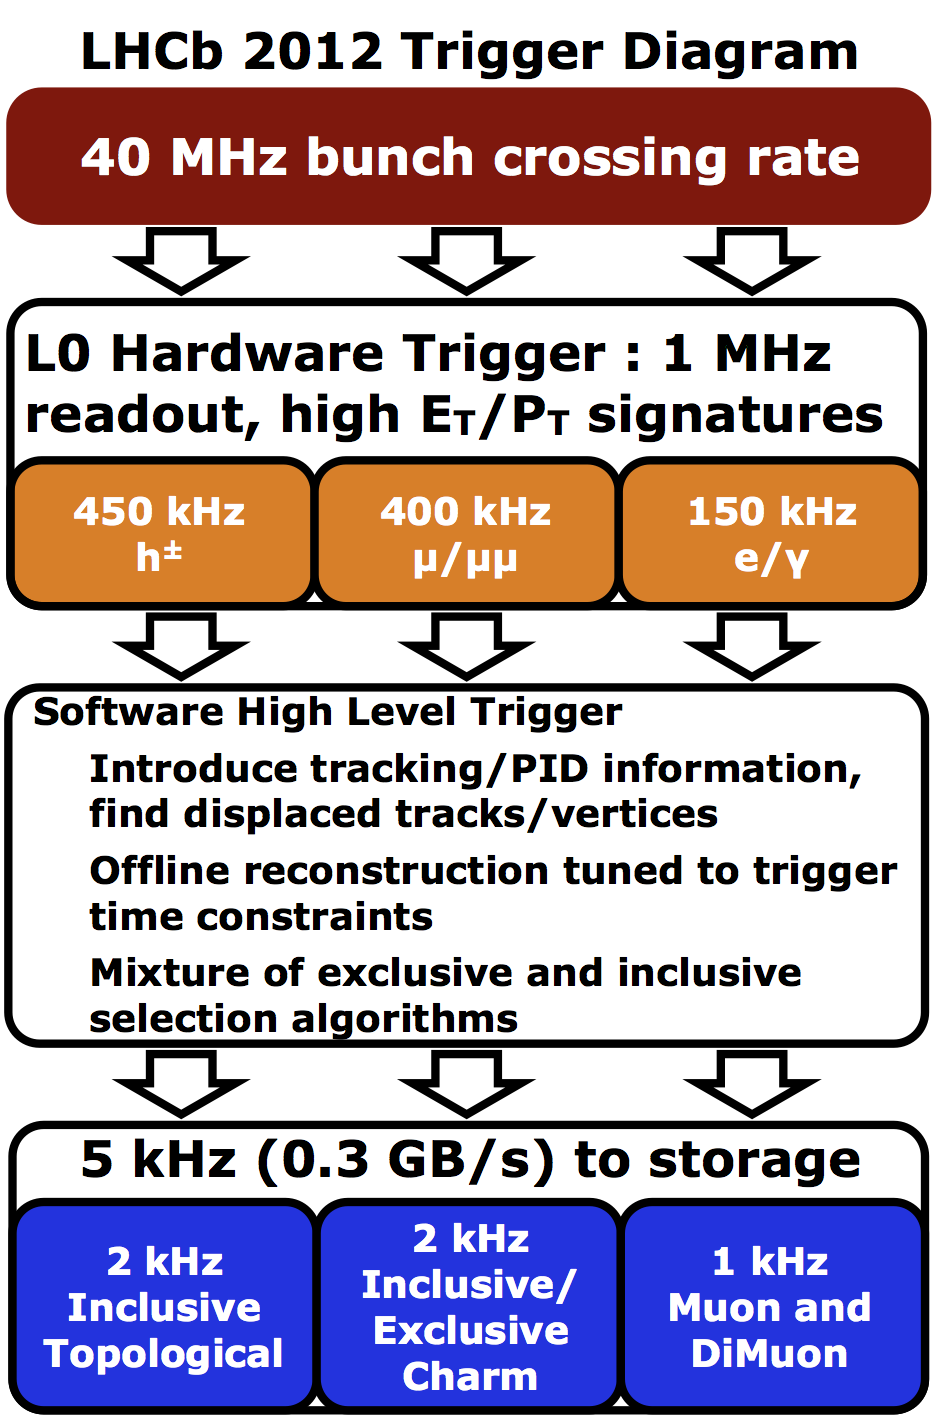
\includegraphics[width=0.45\columnwidth]{figures/detector/Trigger_Run1.png}\hspace{1cm}
    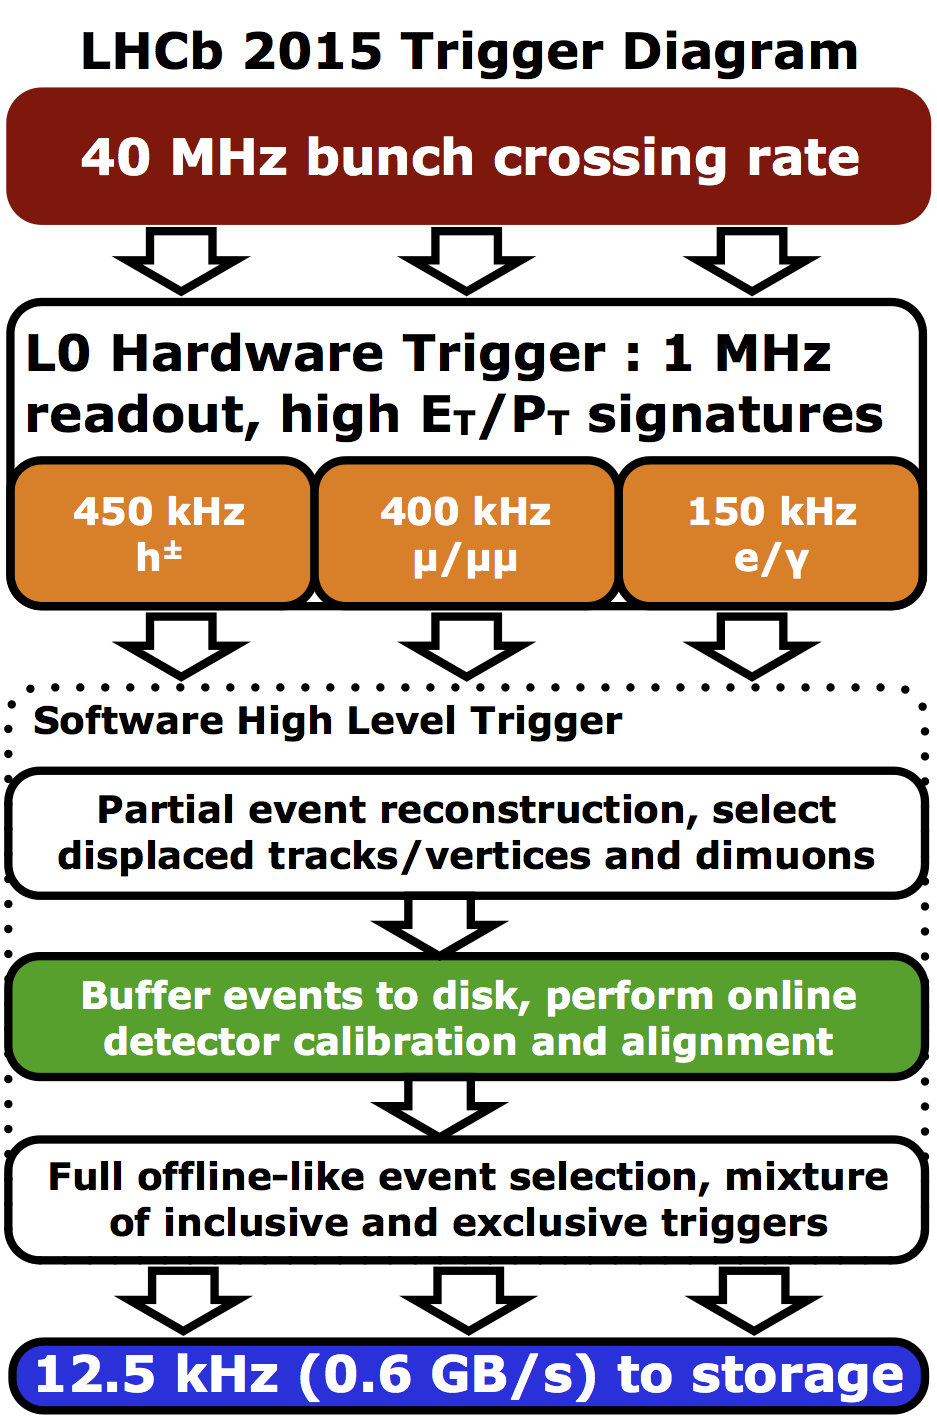
\includegraphics[width=0.45\columnwidth]{figures/detector/Trigger_Run2.png}
    \caption{Illustration of stages and event processing rates in the \lhcb trigger during (left) Run~1 and (right) Run~2. Reproduced from Refs.~\cite{Trigger-Performance,Trigger-Performance2}.}
    \label{fig:trigger_stages}
\end{figure}

The collision rate in the LHC is up to 40\,MHz, with a visible inelastic collision rate in \lhcb of up to 30\,MHz. The \lhcb uses a multi-stage trigger to reduce rate with which events are stored to a manageable level (of eg. 12.5\,kHz during Run~2). The first stage consists of a hardware trigger that selects events with high transverse energy in the calorimeters, or hits in the muon detectors. This is followed by two software stages that rely on a reconstruction of tracks in the detector to select events that are likely to include interesting physics.  The overall trigger stages were identical in Run~1 and Run~2, however the throughput rate was upgraded significantly between the two data taking periods, as was the quality of the reconstruction in the software trigger stages; in Run~2, the final software trigger decisions are in fact based on an event reconstruction that is fully equivalent to the  one performed offline~\cite{Trigger-Performance2}.  The stages are illustrated in Fig.~\ref{fig:trigger_stages}, and described in detail in the following.

A further, offline processing and reconstruction step is applied to all events before they are made available to most \lhcb analyses, commonly denoted as the \emph{stripping} step. Although the stripping does not form part of the \lhcb trigger, it does constitute an additional, centralised filter on the data, and a description is included in Section~\ref{sub:offline_data_filtering_the_lhcb_stripping}.



\subsection{The level-0 hardware trigger} % (fold)
\label{sub:the_level_0_hardware_trigger}

The level-0 (L0) triggers that select physics events are based on the calorimeters and the muon system. 
The ECAL and HCAL are divided into clusters of $2\times2$ cells, for which the transverse energy is defined as
\begin{align}
    E_T=\sum_{j=1}^4 E_j \sin \theta_j,
\end{align}
where $\theta_j$ is the angle of cell $j$ with respect to the beam axis and the average collision point. The trigger forms a \texttt{L0Hadron} candidate with the highest $E_T$ found in the HCAL, combined with the ECAL cluster in front of it if such a cluster is present. Photon and electron candidates are formed based on clusters in the ECAL, identified by the presence (lack) of hits in the SPD for an electron (photon). The transverse energies of the candidates are compared to a fixed set of thresholds, and events where at least one candidate is above threshold are retained.

The muon trigger searches for straight line tracks in the muon stations, estimating the associated muon $p_T$ based on the track direction. An event is retained if either the largest muon $p_T$ is above a given threshold, or the product of the two highest muon $p_T$ values is above a different threshold.

High-multiplicity events take a long time to process in the subsequent software stage; therefore it is favourable for the overall retention rate of interesting physics decays to put a maximum limit on the event multiplicity at the L0 stage. This is achieved by requiring the number of hits in the SPD detector to be below a threshold value in most L0 decisions.

% subsection the_level_0_hardware_trigger (end)

\subsection{High-level triggers} % (fold)
\label{sub:high_level_triggers}

The events that pass the L0 trigger are passed to a farm of multiprocessor computing nodes, the Event Filter Farm (EFF), tasked with bringing the rate down from approximately 1\,MHz to the $\mathcal O(1-10)$\,kHz rate that can be saved to disk. The EFF consisted of 900 (1700) nodes during Run~1 (Run~2). The software-based filtering proceeds in two stages: a first filter (HLT1) brings the rate down to approximately 40\,(110)\,kHz based on a limited reconstruction of the event,  after which a second stage  (HLT2) filters the events further based on a more complete reconstruction. Each step executes a number of different algorithms, each of which can allow an event to be accepted; these are denoted \emph{trigger lines.}

During both runs, the HLT1 performed a partial event reconstruction by building long tracks that satisfy a $p_T$ requirement using the forward tracking approach described in Section~\ref{sub:track_reconstruction}, and determining the location of PVs using VELO tracks. In both runs, the HLT1 included an inclusive trigger that selected a high $p_T$ track with significant displacement of all PVs (typical of a $b$ or $c$ decay). This line is denoted \texttt{HLT1TrackAllL0} in Run~1~\cite{Trigger-Performance}; for Run~2 the track requirements were reoptimised and it is denoted \texttt{Hlt1TrackMVA}. Further, an additional inclusive trigger was added that forms a two-prong vertex out of high $p_T$ tracks inconsistent with originating in a PV, and applies a multivariate classifier to determine if it is signal-like based on a number of track and vertex properties. This line is denoted \texttt{Hlt1TwoTrackMVA}~\cite{Trigger-Performance2}. These lines triggered all events included in the analysis of the thesis; other lines exist for selecting events that include muons, calibration data, low-multiplicity events, and a number of exclusive lines, for a total of approximately 20 lines during Run~2~\cite{Trigger-Performance2}.

The rate of events is reduced significantly by HLT1, and therefore the HLT2 decisions can be based on a more complete reconstruction of the event. Indeed, during Run~2 it was based on a complete, fully aligned reconstruction equivalent to the offline reconstruction. During Run~1 the HLT2 reconstruction only included long tracks and did exclude some low momentum tracks; this was a main motivation for the upgrade of the EFF during the shutdown period. The need for full alignment in HLT2 means that it could not be run fully online in Run~2; instead the output events from HLT1 were saved to disk in the EFF, and processed with some delay~\cite{Trigger-Performance2}. The analysis presented in the thesis is based on a number of inclusive "topological" trigger lines, based on combinations of 2, 3, or 4 tracks that satisfy fit quality requirements, have high $p_T$, are separated from the PVs, and have a distance-of-closes-approach below 0.2\mm. A multivariate classifier~\cite{gligorovEfficientReliableFast2013} is applied to each formed $n$-body object, to determine if the event should be accepted based on the track momenta, invariant mass, a corrected invariant mass that takes into account missing transverse momentum, distance of closest approach, and the impact parameter and separation with the associated PV. The resulting trigger lines were denoted \texttt{Hlt2Topo\{2, 3, 4\}BodyBBDT} during Run~1 and \texttt{Hlt2Topo\{2, 3, 4\}Body} during Run~2.  A large number of other HLT2 lines exist (more than 500 in Run~2), including a significant number of exclusive lines that aim to select specific decays and only save information on the signal decay, not the whole event. This was made possible by the full reconstruction within HLT2~\cite{Trigger-Performance2}, and have allowed for larger signal yields to be collected within the data storage limits.

% subsection high_level_triggers (end)

\subsection{Offline data filtering: the \lhcb stripping} % (fold)
\label{sub:offline_data_filtering_the_lhcb_stripping}

Events that are written to disk are processed with the full detector alignment and calibration. In a further, offline processing step denoted the \emph{stripping}, hundreds of different, dedicated reconstructions are performed; decay candidates for various signal decays are built and a number of requirements are made to reject backgrounds from random track combinations. For example, the $\Bpm\to\D(\to\KS h'^+h'^-)h^\pm$ candidates that are analysed in this thesis are built during the stripping stage, as described further in Section~\ref{sec:candidate_selection}. The stripping is a centralised computing task, executed on the Worldwide LHC Computing Grid~\cite{birdComputingLargeHadron2011a}, and allows the analysts to process much smaller data sets during their individual analysis. Because the stripping is based on data saved to offline storage it can be repeated; however, the processing of data collected during a year of data taking takes many weeks, so this does not happen often.

% subsection offline_data_filtering_the_lhcb_stripping (end)

% section the_lhcb_triggerring_system (end)



\section{Simulation} % (fold)
\label{sec:simulation}

A centralised \lhcb simulation is able to simulate $pp$ collisions with the proper conditions within \lhcb, model subsequent secondary decays and the full detector response, and process the output in the full \lhcb reconstruction. In this thesis, simulated decays are used to determine the reconstructed invariant-mass distribution of a number of decay modes, as well as a number of relative selection efficiencies. The $pp$ collisions are generated using \pythia~\cite{Sjostrand:2007gs,*Sjostrand:2006za} with a configuration specific to \lhcb~\cite{LHCb-PROC-2010-056}. The time-dependent evolution and decays of unstable particles are described by the \evtgen~\cite{EvtGen} package, designed specifically for \B physics. Final-state radiation is generated using \photos~\cite{Golonka:2005pn}. The interaction of the generated particles with the detector, and its response, are implemented using the \geant toolkit~\cite{Allison:2006ve, *Agostinelli:2002hh} as described in  Ref.~\cite{LHCb-PROC-2011-006}. 

The most significant computational cost of the simulation is due to the detector simulation. A single $pp$ collision produces $\mathcal O(100)$ tracks in the detector, out of which only a handful belong to the signal decay under study. Therefore, significant computational resources can be saved by reusing the detector simulation of non-signal tracks a number of times, while redecaying the signal particle, say a \Bp, each time. This approach is called ReDecay~\cite{LHCb-DP-2018-004}, and has been relatively widely adopted within \lhcb. ReDecay has been used to produce simulation samples corresponding to the conditions in 2017 and 2018 for this thesis. In some cases, the use of ReDecay necessitates special statistical treatment due the correlated detector occupancies between signal candidates, but for the analysis in this thesis the impact is negligible.

A number of sub-dominant backgrounds are investigated using the fast-simulation package \texttt{RapidSim}~\cite{cowanRapidSimApplicationFast2017}. This package can decay heavy $b$ and $c$ hadrons with kinematic distributions similar to those in \lhcb $pp$ collisions, or with user defined input distributions. The decays are typically evenly distributed over phase space, but can also be handled with \evtgen~\cite{EvtGen} to take involved a given resonant structure into account. Furthermore, a smearing of the obtained momenta can be applied that is based on the \lhcb resolution. 

% subsection rapidsim_a_fast_simulation_tool (end)RapidSim.

\section{Data-taking conditions} % (fold)
\label{sec:past_and_future_data_taking_conditions}

\begin{table}[tp]
    \centering
    \caption{Overview of the running condition and collected data samples by the \lhcb experiment during Run~1~and~2 of the LHC~\cite{LHCbLumi}. A brief overview of data taking periods planned for the future is also shown.\label{tab:run_conditions}}
    \begin{tabular}{cccc}
    \toprule
    LHC phase   & Year  & $\sqrt s / \tev$  & $\int \mathcal L\,\mathrm dt$ / \invfb \\
    \midrule
    Run 1       & 2011  & 7                 & 1.0 \\
                & 2012  & 8                 & 2.0 \\
    \midrule
    Run 2       & 2015  & 13                & 0.3 \\
                & 2016  &                   & 1.6 \\
                & 2017  &                   & 1.7 \\
                & 2018  &                   & 2.1 \\
    \bottomrule
    \end{tabular}
\end{table}



The \lhcb experiment has collected a data set corresponding to to 8.7\invfb during Run~1 and 2 of the LHC. The running conditions for each year are summarised in Table~\ref{tab:run_conditions}. The measurement that is the main topic of the thesis is based on the full data set.

The $\Bpm$ production cross section increased significantly with the higher centre-of-mass energy during Run~2. In the \lhcb acceptance, the cross section has been measured to be approximately 43\,$\mu$b at $\sqrt s =7\tev$, increasing to about 87\,$\mu$b at $\sqrt s =13\tev$~\cite{LHCb-PAPER-2017-037}. In combination with an increased selection efficiency due to improvements to the trigger, this resulted in signal yields per \invfb that were about 2.5 times higher in Run~2 than in Run~1, in the measurement described in Chapter~\ref{ch:5-GGSZ-measurement}. Before delving into the details of that analysis, Chapter~\ref{ch:4-KS-CPV} is dedicated to a phenomenological study of how it is impacted neutral kaon \CP violation and interaction with the \lhcb detector.

% section past_and_future_data_taking_conditions (end)

% section simulation (end)